\documentclass[10pts]{article}
\usepackage{times}
\usepackage{epsfig}
\usepackage{graphicx}
\usepackage{natbib}
\usepackage{hyperref}

\addtolength{\textwidth}{2cm}
%\addtolength{\textwidth}{1cm}
\addtolength{\textheight}{2cm}
%\addtolength{\textheight}{1cm}
\addtolength{\topmargin}{-1cm}
\addtolength{\oddsidemargin}{-1cm}
\addtolength{\evensidemargin}{-1cm}

\newcommand{\deri}[2]{\frac{\partial  #1}{\partial #2}}

\parskip 0.1in
\parindent 0.0in
\setcounter{secnumdepth}{1}
\title{Deep Learning}

\author{Yann LeCun, Yoshua Bengio, Geoffrey Hinton}

\begin{document}

\maketitle

\section{Preface}

Deep Learning techniques allow a machine composed of multiple layers
of processing to learn to represent data, so that each layer transforms
the representation of the previous layer in a more abstract
fashion. These methods have dramatically improved the state-of-the-art
for speech recognition, object recognition, object detection,
predicting the activity of drug molecules, and many other tasks. Deep
learning discovers intricate structure in large datasets by using the
{\em backpropagation algorithm} to compute how the machine should
change in order to make less errors.  Deep {\em convolutional nets}
have brought about dramatic improvements in the processing of array
data, such as images, video, speech and audio, while {\em recurrent
  nets} have shown excellent performance for analyzing sequential
inputs and producing sequential outputs such as text and
speech. Convolutional nets have quickly become the leading technology for image
recognition and speech recognition, while recurrent nets are
competitive in several natural language processing tasks, including
language translation. Combinations of recurrent and convolutional nets
can generate good textual captions of images.

\section{Introduction}

% what is machine learning
Machine learning technology (ML) powers many aspects of modern
society: from web search to content filtering on social networks, and
to recommendations on e-commerce websites. It is also increasingly
present in consumer products such as cameras and smartphones. ML
systems are used to identify objects in images, transcribe speech into
text, match news items, posts, or products with users' interests, and
select relevant results of search. Increasingly, these applications
make use a new class of techniques: {\em deep learning}.

% handcrafted features
Traditional ML techniques are limited in their ability to process
natural data in raw form. For decades, constructing a pattern
recognition or ML system has required engineering efforts and domain
expertise to design a {\em feature extractor} that transforms the raw
data, such as the pixel values of an image, into a suitable {\em
  internal representation}, or feature vector, from which the learning
subsystem, often a classifier, can detect, recognize, or classify
patterns in the input.

% deep learning: learning representations
Deep learning is a set of methods that allows a machine to be fed with
raw data and to automatically discover suitable representations of the
data. The name comes from the fact that deep learning machines are
multilayer stacks of trainable modules, each of which turns the
representation of the data in its input into a more abstract and
higher-level representation on its output in which relevant
characteristics and amplified and irrelevant variabilities are
attenuated. For example, an image comes in the form of an array of
pixel values, features in the first layer would represent the presence
or absence of edges of a particular orientation at all locations in
the image, the second layer would  detect motifs by spotting particular
arrangements of edges, regardless of small variations in the positions
of the edges.  The third layer would assemble motifs into parts of
object, and subsequent layers would to detect objects as combinations of
parts. The key aspect of deep learning is that {\em these features and
  representations are not designed by human engineers, but are
  automatically learned from data.}

% preview of deep learning results
Deep learning is making major advances in solving problems that have
resisted the best attempts of the Artificial Intelligence community
for many years. It has turned out to be very good at discovering
intricate structure in large, high-dimensional data and is therefore
applicable to many domains of science, business, and government. In
addition to beating records in image
recognition~\citep{Krizhevsky-2012-small,farabet-pami-13,tompson-nips-14,szegedy-2014}
and speech
recognition~\citep{Hinton-et-al-2012,Sainath-et-al-ICASSP2013}, it has
beaten other ML techniques at predicting the activity of potential
drug molecules~\citep{Dahl-et-al-arxiv2014}, detecting new fundamental
particles~\citep{Melis-Higgs-boson-competition-2014},
%~\citep{YANNparticles} % YB while waiting for bib entry, 
% classifying galaxies, ~\citep{YANNgalaxies}, % YB while waiting for bib entry, 
reconstructing brain circuits~\citep{helmstaedter-nature-2013}, and
predicting the effects of mutations in non-coding DNA on gene
expression and disease~\citep{Keung-et-al-2014}.

Perhaps more interestingly, deep learning has produced extremely
promising results for a variety of tasks in natural language
understanding~\citep{collobert:2011b}, particularly topic
classification, %~\citep{topic-classification},  % YB while waiting for bib entry
sentiment
analysis~\citep{Glorot+al-ICML-2011-small},
question-answering~\cite{Bordes-et-al-EMNLP2014}, and language
translation~\cite{Jean-et-al-arxiv2014,Sutskever-et-al-NIPS2014}.


% supervised learning, objective function, gradient.
The most common form of machine learning, deep or not, is {\em
  supervised learning}. Imagine that we want to build a system that
can classify images as containing, say, a house, a car, a person, or a
pet. We first collect a large dataset of images of houses, cars,
persons and pets, each labeled with its category. During training, the
machine is shown an image and produces an output in the form of
a vector of scores, one for each category. We want the desired
category to have the highest score of all categories, but this is
unlikely to happen before training.  We compute an {\em objective
  function}, that measures the error (or distance) between the output
scores and the desired pattern of scores. The machine then modifies
its internal adjustable parameters so as to reduce this error. These
adjustable parameters, often called weights, are real numbers which
can be seen as ``knobs'' that define the input-output function of the
machine. In a typical deep learning system, there may be hundreds of
millions of these adjustable weights, and tens or hundreds of millions
of examples with which to train the machine.

To properly adjust the weight vector, the learning algorithm computes
a {\em gradient vector} which, for each weight, indicates by what
amount the error would increase or decrease if the weight were
increased by a tiny amount. The weight vector is then adjusted in the
opposite direction of the gradient vector. 

% GD
The objective function, averaged over all the training examples, can
be seen as a kind of hilly landscape in the high-dimensional space of
weight values. The negative gradient vector indicates the direction of
steepest descent in this landscape, taking it closer to a minimum
where the output error is low on average.

% SGD
In practice, most practitioners use a procedure called {\em Stochastic
  Gradient Descent} or SGD. It consists in showing an input, computing
the output and the error, computing the gradient, and adjusting the
weight vector right away. The process is repeated with each example in
the training set, again and again, until the average of the objective
function stops decreasing. It is called stochastic because each sample
gives a noisy estimate of the average gradient. The procedure gets
close to a good minimum very quickly in
practice~\cite{bottou-bousquet-2008-small}. Following this, the
performance of the system is measured on a different set of examples,
not seen during training, called a {\em test set}. This serves to test
the {\em generalization ability} of the machine, i.e. its ability to
produce sensible answers on new inputs that it has never seen during
training.

% shallow linear classifiers
Many practical applications of ML use linear classifiers on top of
hand-engineered features. A two-class linear classifier computes a
weighted sum of the feature vector components. If the weighted sum is
above a threshold, the input is classified as belonging to a
particular category. Multiple classes can be handled by using multiple
two-class classifiers, each classifying one class against all
others. The learning procedure adjusts the weights of the linear
combination, for which the gradient is very easy to compute. Linear
classifiers have been widely used for many decades, starting with the
Perceptron model~\citep{Rosenblatt57}, the still-popular logistic
regression~\cite{Hastie2001}, and the linear support vector
machine~\cite{Boser92}. 

% features: solving the selectivity-invariance dilemma
It has been known since the 1960s that linear classifiers can only
carve out their input space into very simple regions, namely
half-spaces separated by a hyperplane~\citep{Duda-Hart}.  But problems
such as image and speech recognition require the input-output function
to be insensitive to irrelevant variations of the input, such as
variations in position, orientation or illumination of an object, or
variation in pitch or accent of speech, while being very sensitive to
particular minute variations, such as the difference between a white
wolf and a samoyed (a breed of wolf-like white dog).  At the pixel
level, images of two samoyeds in different poses and in different
environments may be very different from each other, while two images
of a samoyed and a wolf in the same position and on similar
backgrounds may be quite similar to each other. A linear classifier,
or any other ``shallow'' classifiers operating on raw pixels could not
possibly distinguish the latter two, while putting the former two in
the same category. This is why shallow classifiers require a good
feature extractor that solve the {\em selectivity-invariance dilemma},
i.e. that produces representations that are {\em selective} to the
important aspects of the image, while being {\em invariant} to its
irrelevant aspects, like the pose of the animal.

% classical extensions of simple classifiers
There have been numerous attempts, going back to the early 1960s, to
increase the flexibility of classifiers so as to allow them to
separate categories from one another by more complex surfaces than
flat hyperplanes. A popular example is the class of kernel methods,
particularly the Support Vector Machine~\citep{Boser92} which
represents inputs by a vector whose components are similarities to
each of the training samples computed through a so-called {\em kernel
  function}. While these methods are good general-purpose classifiers,
they do not perform well for tasks such as image or speech recognition
in which the input space is very high-dimensional and the input-output
mapping is so complex that computing similarities using a simple
kernel function is ineffective. Designing feature extractors that are
sensitive to the relevant information and invariant to the irrelevant
one is what generations of computer vision and pattern recognition
researchers have spent their careers on.

% deep architectures
But what if features could be learned? That is the key idea of deep
learning.

A deep learning architecture is a multilayer stack of modules, all (or
most) of which are subject to learning, and many of which compute
non-linear input-output mappings.  Each module in the stack transforms
its input so as to increase both the selectivity and the invariance a
little bit.  With multiple non-linear layers, say 5 to 20, a system
can implement extremely intricate functions of its inputs that are
simultaneously sensitive to minute details-- distinguishing samoyeds
from wolves-- and insensitive to irrelevant variations such as the
background, the pose, the lighting, or the surrounding objects.

% backprop
How do we train multilayer architectures? 

From the earliest days of pattern
recognition~\citep{selfridge,Rosenblatt57} researchers have aimed to
replace hand-engineered features by trainable multilayer networks.
But despite its extreme simplicity, the solution did not appear until
the mid 1980s and was largely forsaken by the ML community until
recently. As it turns out, training multilayer architectures can be
done by simple stochastic gradient descent. As long as the modules are
relatively smooth functions of their inputs and of their internal
weights, one can compute gradients through the {\em backpropagation
  procedure}.

The idea that this could be done, and that it could work at all, took
a surprisingly long time to emerge. It was discovered independently by
everal different groups in the 1970s and
1980s~\citep{Werbos74,Parker85,LeCun85,RHW}, and became quite popular
in the late 1980s, spurring the second wave of interest for neural
networks. But for reasons that historians of science will have to
explain, the method was the subject of scorn by the ML community
between the late 1990s and the late 2000s.

The backpropagtion procedure to compute gradient of an objective
function with respect to the weights of a multilayer stack of modules
is nothing more than a practical application of the chain rule for
derivatives. The key insight is that the derivative (or gradient) of
the objective with respect to the {\it input} of a module can be
computed by working backwards from the gradient with respect to the
{\em output} of that module (or the input of the subsequent
module). Basically, take a module $M$ inside the network, whose input
is $x$, weight vector is $w$, and output is $y = M(x,w)$. If one knows
the gradient $\deri{E}{y}$ of the objective function $E$ with respect
to the module's output $y$, one can blindly apply chain rule to
compute the gradient with respect to the input:
\[
  \deri{E}{x} = \deri{y}{x}\deri{E}{y}
\]
This equation works even when $x$ and $y$ are vectors, in which case
$\deri{E}{x}$ and $\deri{E}{y}$ are gradient vectors, and
$\deri{y}{x}$ is a {\em Jacobian matrix} of $M$ where element $(i,j)$
indicates by how much output $j$ would increase proportionally if
input $i$ were increased by a tiny amount $\Delta y_j =
\left(\deri{y}{x}\right)_{ij} \Delta x_i$. The above equation
constitutes a recurrence formula that can be used to propagate
gradients from the top layer all the way to the bottom. Once all these
gradients are computed, one can similarly compute the gradients with
respect to the weights of the module. Figure~\ref{fig:backprop-box})
shows how this works out when the network is composed of layers of
weight matrices interspersed with scalar non-linearities.
%% the notation in the figure should be updated.


% deep neural nets
Many applications of deep learning use feedforward neural network
architectures, illustrated in Figure~\ref{fig:backprop-box}, which
learn to map a fixed-size input (e.g., an image) to a fixed-size
output (e.g. a probability for each one of several categories). To go
from one layer to the next, a set of units compute a weighted
sum of their inputs from the previous layer and pass the result
through a non-linear function. The most common non-linear function is
the so-called {\em ReLU} (Rectified Linear Unit) which is simply the
half-wave rectifier $f(z) = \max(z,0)$. In past decades, neural nets
used smoother non-linearities, such as $\tanh(z)$, but the ReLU seems
to work better in networks with many layers. Units that are not in the
output layer are traditionally called {\em hidden units}. The first
layers can be seen as distorting the input in a non-linear way so that
categories become linearly separable by the last layer, as indicated
in figure~\ref{fig:backprop-box}.



\begin{figure}[htp]
\fbox{
\begin{minipage}{\textwidth}
\centerline{
\fbox{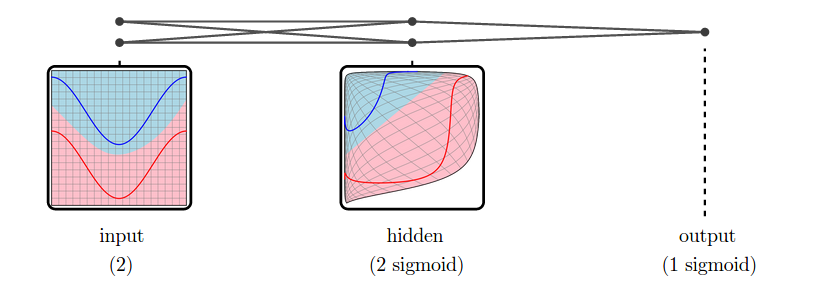
\includegraphics[width=0.69\linewidth]{netvis-simple-2S.png}}
\fbox{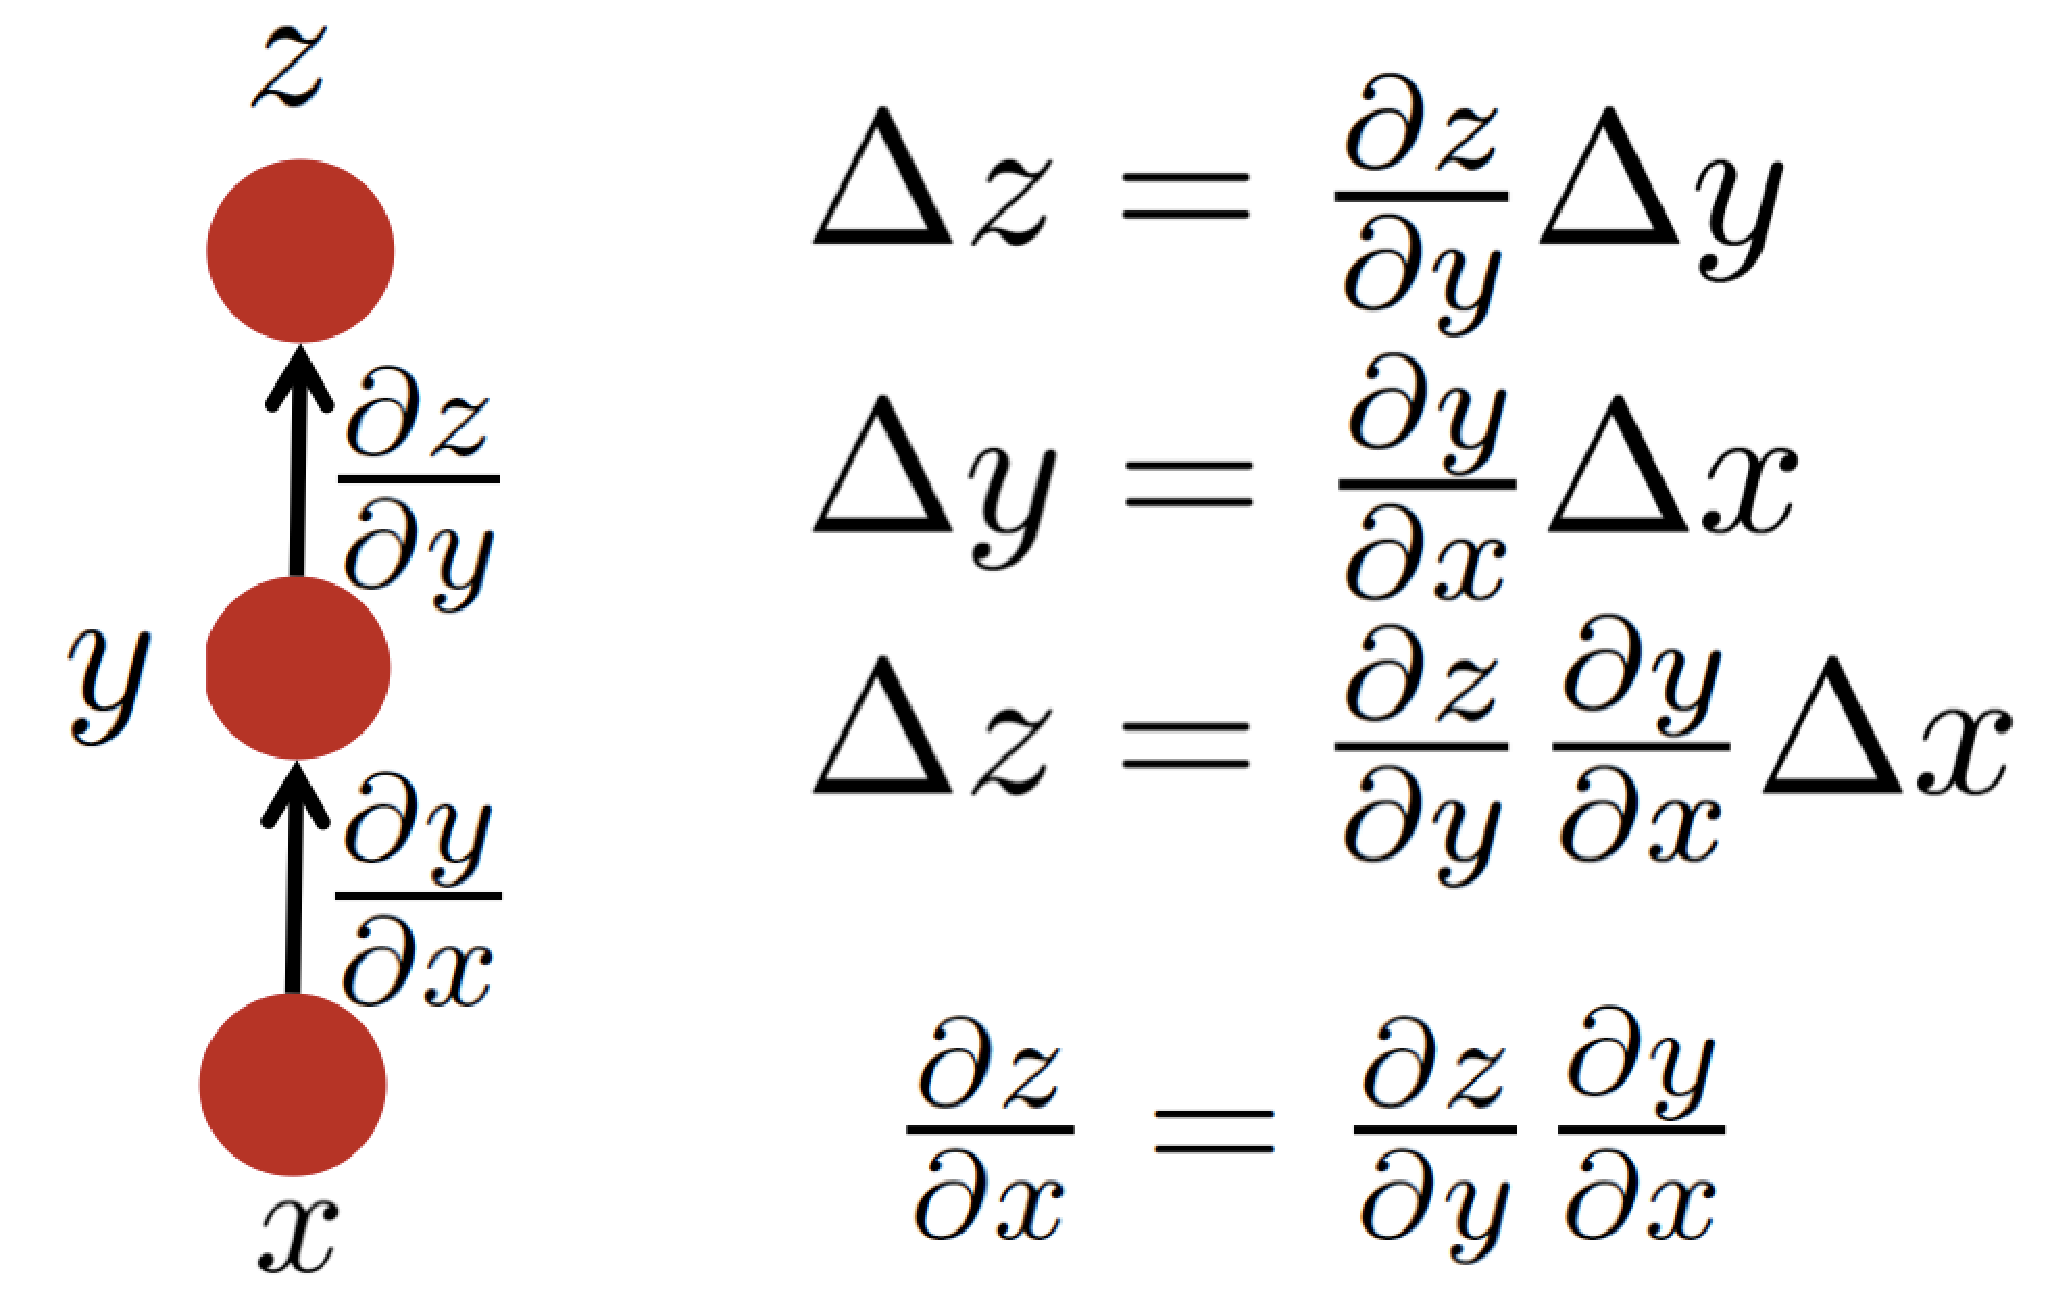
\includegraphics[width=0.28\linewidth]{chain-rule.pdf}}}
\centerline{
\hspace*{.5mm}\fbox{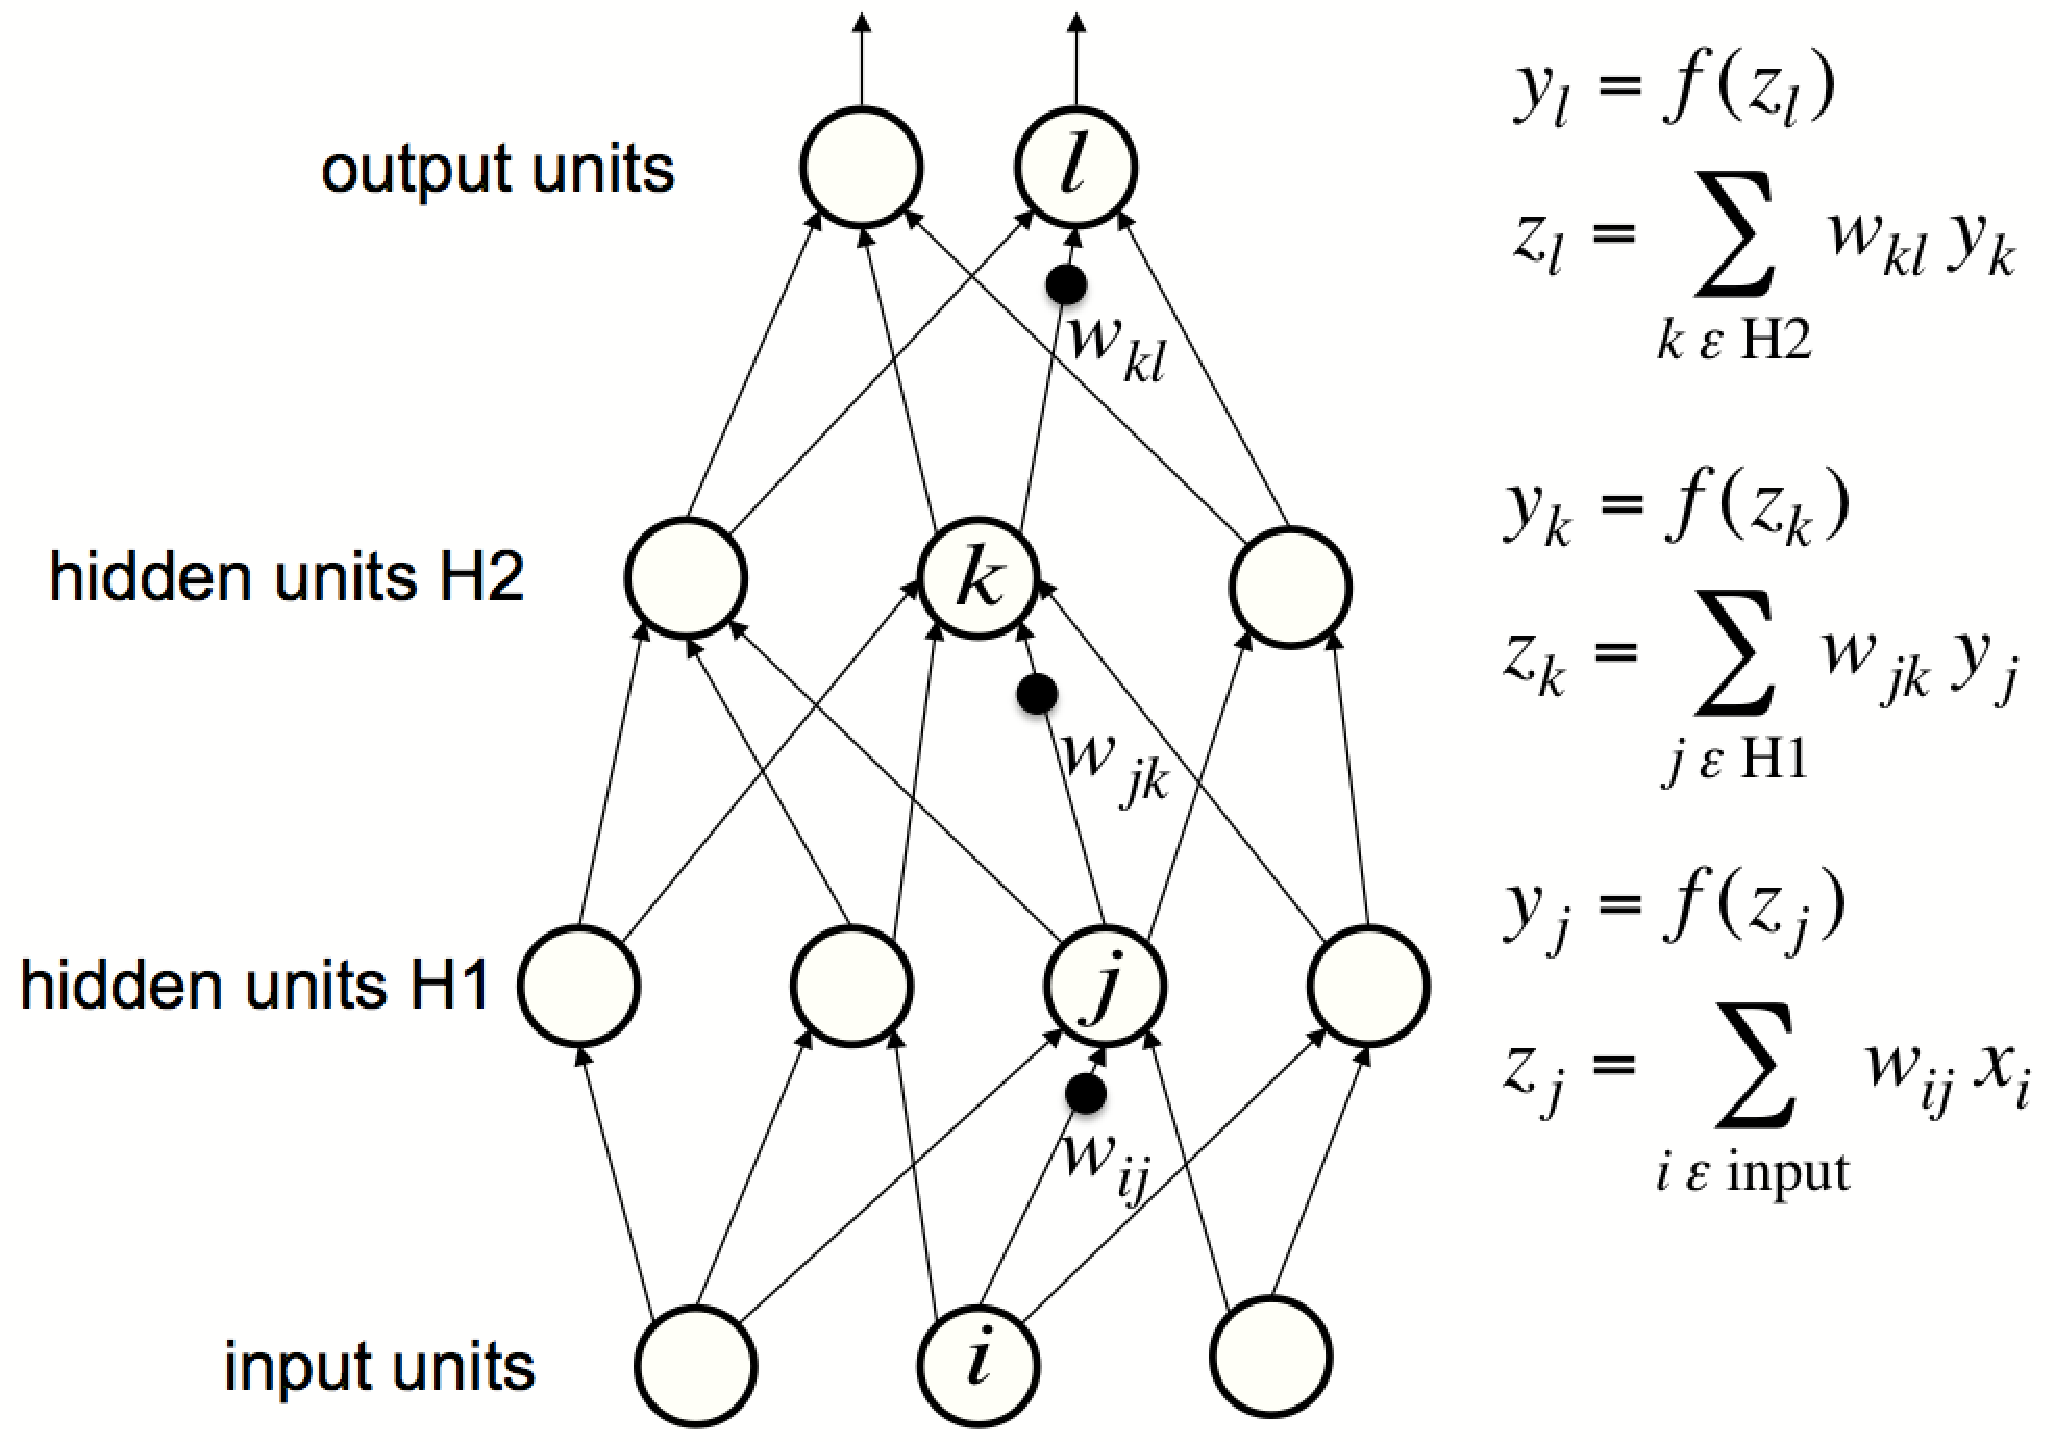
\includegraphics[width=0.49\linewidth]{bpfig_forward.pdf}}
\hspace*{0mm}\fbox{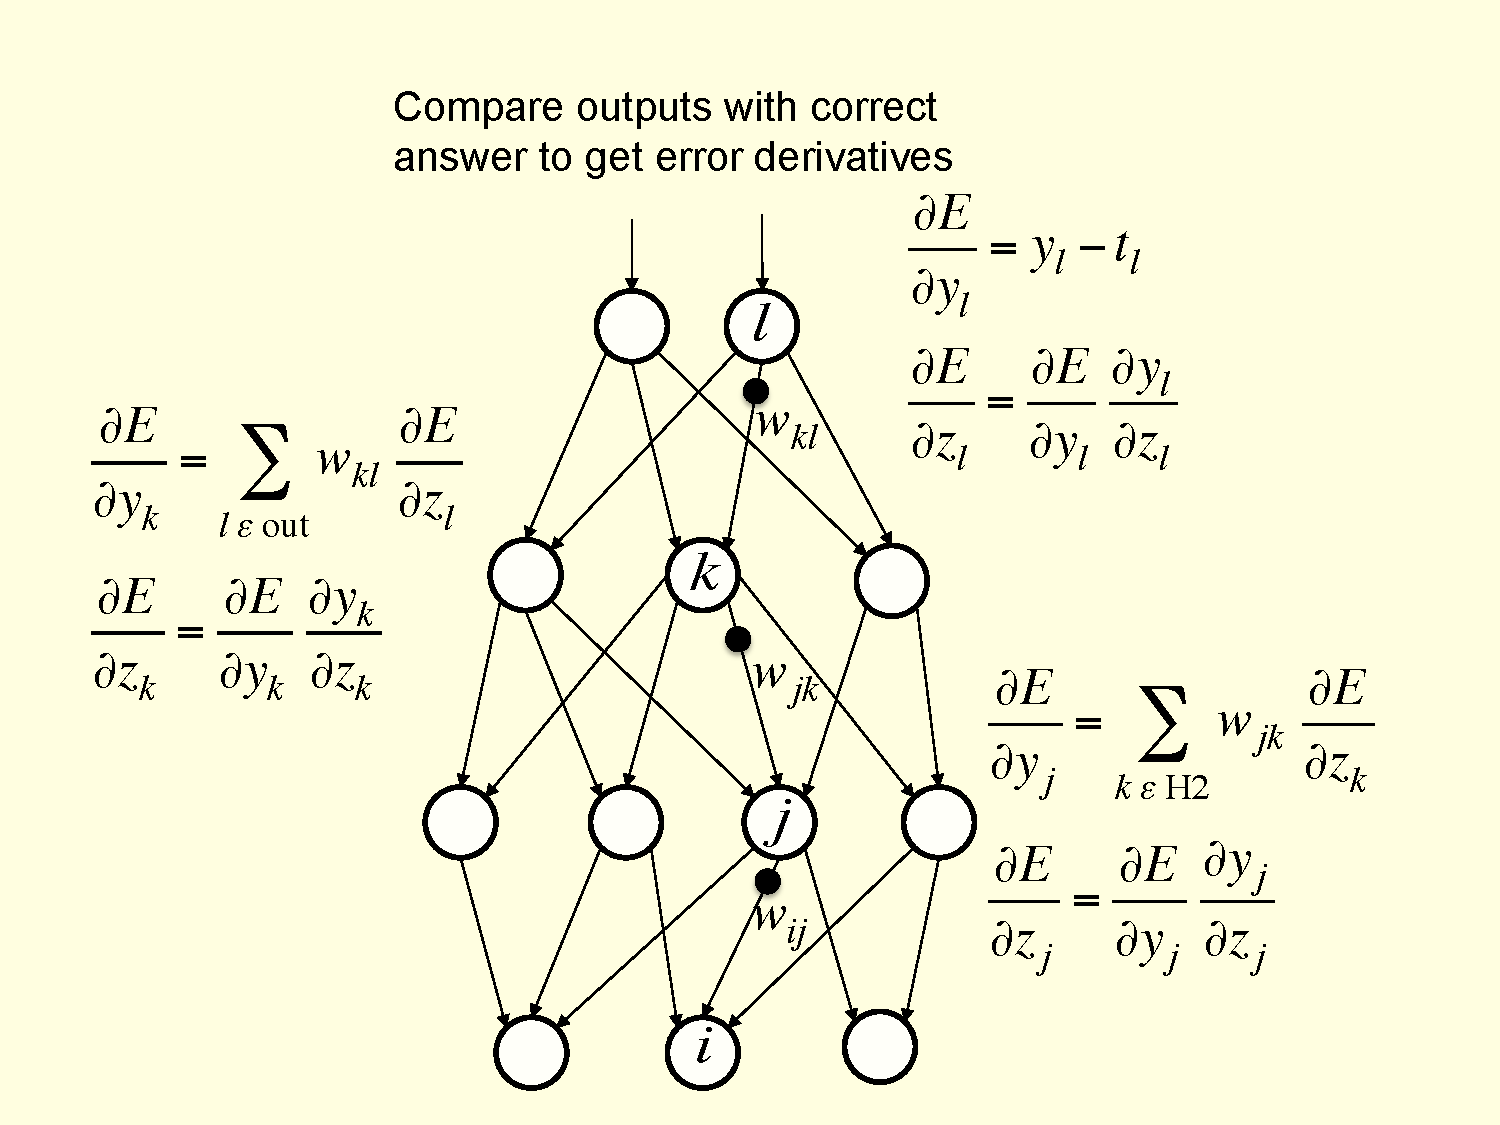
\includegraphics[width=0.49\linewidth]{bpfig_backward.pdf}}
}
\caption{
{\bf Top left.} A multi-layer neural network can distort the
input space to make the classes (whose examples are supposed to
be on the red and blue lines, here) linearly separable. Note how
a regular grid in input space is also transformed. This is an
illustrative example with only two input units, two hidden units
and one output unit, but the networks used for object recognition
or natural language processing contain tens or hundreds of thousand
of units. Reproduced with permission by Chris Olah from~\url{http://colah.github.io/}.
\newline
{\bf Top right.} The chain rule of derivatives tells us how
two small effects (that of a small change of $x$ on $y$, and that of $y$ on $z$)
are composed. A small change $\Delta x$ in $x$
gets transformed first into a small change $\Delta y$ in $y$
by getting multiplied by $\frac{\partial y}{\partial x}$
(that is the definition of partial derivative). Similarly,
the change $\Delta y$ creates a change $\Delta z$ in $z$. Substituting one equation
into the other gives the chain rule of derivatives, i.e., how
$\Delta x$ gets turned into $\Delta z$ through multiplication
by the product of $\frac{\partial y}{\partial x}$ and
$\frac{\partial z}{\partial x}$. It also works when $x$, $y$
and $z$ are vectors (and the derivatives are Jacobian matrices). 
\newline
{\bf Bottom left.} 
The equations used for computing the forward pass in a neural
net with two hidden layers. At each layer, we first compute the total
input $z$ to each unit, which is a weighted sum of the outputs of the
units in the layer below. Then a non-linear function $f(.)$ is applied
to $z$ to get the output of the unit.  For simplicity, we have omitted
bias terms. The non-linear function used in neural networks include 
the rectified linear unit (ReLU) $f(z) = max(0, z)$, commonly-used in 
recent years, as well as the more traditional sigmoids, such as the 
hyberbolic tangent, $f(z) = (\exp(z)-\exp(-z))/(\exp(z)+\exp(-z))$ 
and logistic function logistic, $f(z) = 1/(1+\exp(-z))$.
{\bf Bottom right.} 
The equations used for computing the backward pass. At each
hidden layer we compute the error-derivative w.r.t. the output of each
unit which is a weighted sum of the error-derivatives w.r.t. the total
inputs to the units in the layer above. We then convert the
error-derivative w.r.t. the output into the error-derivative w.r.t.
the input by multipling it by the gradient of $f(z)$.  At the output
layer, the error-derivative w.r.t. the output of a unit is computed by
differentiating the cost function. This gives $y_l-t_l$ if the cost
function for unit $l$ is $0.5(y_l-t_l)^2$ where $t_l$ is the target
value. Once the $\partial E/\partial z_k$ is known, the
error-derivative for the weight $w_{jk}$ on the connection from unit
$j$ in the layer below is just $y_j \partial E/\partial z_k$.
}
\label{fig:backprop-box}
\end{minipage}
}
\end{figure}


\section{Convolutional networks}


\begin{figure}
\begin{center}
  \vspace{0.2cm}
  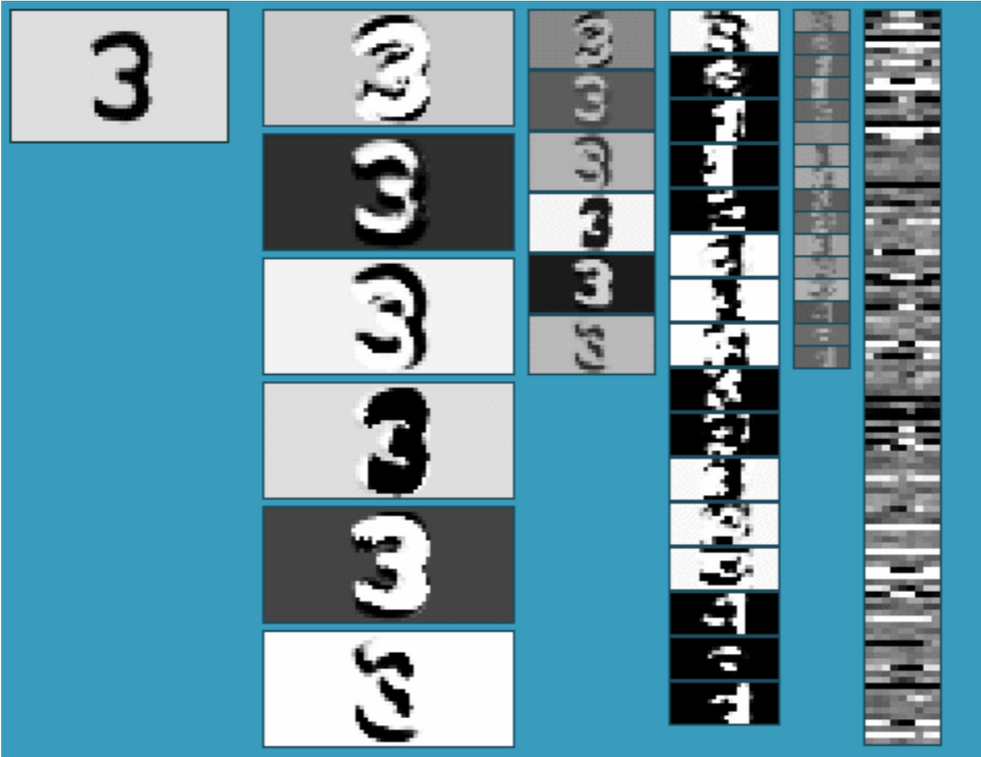
\includegraphics[width=0.70\linewidth]{convnet-diagram}
\end{center}
\vspace{-0.6cm}
\caption{The outputs of each layer of a typical convolutional network architecture
applied on the image of a handwritten digit (on the top left). Each rectangular
image corresponds to one of the features, detected at each of the image positions.
Each column corresponds to a layer, with information flowing from the left to
the right.
}
%\vspace{-0.8cm}
\label{fig:convnet}
\end{figure}

One of the most widely used deep learning architectures is the
convolutional neural network, or
ConvNet~\cite{lecun-90c,lecun-98}. ConvNets are designed to process
data that come in the form of multiple arrays, for example a color
image composed of three 2D arrays containing pixel intensities in the
three color channels. Many data modalities are in the form of multiple
arrays: 1D for signals and sequences including language, 2D for images
or audio spectrograms, 3D for video or volumetric images.  There are
four key ideas behind ConvNets that take advantage of the properties
of many such natural signals: local connections, shared weights,
pooling, and the use of many layers.

The architecture of a typical ConvNet is shown in
figure~\ref{fig:convnet}.  It is structured as a series of stages. The
first few stages are composed of two types of layers: convolutional
layers and pooling layers. Units in a convolutional layer are
organized in {\em feature maps}, within which each unit is connected
to local patches in the feature maps of the previous layer through a
set of weights called a {\em filter bank}. The result of this local
weight sum is then passed through a non-linearity such as a ReLU.  All
units in a feature map share the same filter bank. Different feature
maps in a layer use different filter banks. The reason for this
architecture is twofold. First, in array data such as images, local
groups of values are often highly correlated forming distinctive local
motifs that are easily detected. Second, the local statistics of
images and other signals are invariant to location. In other word, if
a motif can appear in one part of the image, it could appear anywhere,
hence the idea of units at different locations sharing the same
weights, and detecting the same pattern in different parts of the
array.  Mathematically, the filtering operation performed by a feature
map is a {\em discrete convolution}, hence the name ConvNet.

While the role of the convolutional layer is to detect local
conjunctions of features from the previous layer, the role of the
pooling layer is to merge semantically similar features into
one. Since the relative positions of the features forming a motif can
vary somewhat, reliably detecting the motif can be done by
coarse-graining the position of each feature. A typical pooling unit
computes the max of a local patch of units in one feature map (or in a
few feature maps). Neighboring pooling units take input from patches
that are shifted by more than one row or column, thereby reducing the
dimension of the representation and creating an {\em invariance} to
small shifts and distortions.  Two or three stages of convolution,
non-linearity, and pooling are stacked, followed by more convolutional
and fully-connected layers.  Back-propagating gradients through a
ConvNet is as simple as through a regular deep network, allowing all
the weights in all the filter banks to be trained. The error
derivative for a shared weight is just the sum the derivatives for all
the instances of that weight.

This ConvNet architecture exploits the property that many natural
signals are {\em compositional hierarchies}. In images, local
combinations of edges form motifs, motifs assemble into parts, and
parts form objects in various combinations.  Similar hierarchies
exists in speech and text from sounds to phones, phonemes, syllables,
words, and sentences. The pooling allow features that form elements at
the next level to vary in relative position and appearance. 

The convolutional and pooling layers in ConvNets are directly inspired
by the classic notions of simple cells and complex cells in visual
neuroscience~\citep{Hubel62}, and the overall architecture is
reminiscent of the LGN-V1-V2-V4-IT visual cortex ventral pathway
hierarchy ~\citep{Felleman+VanEssen-1991}. When ConvNet models and
monkeys are shown the same picture, the activations of high-level
units in the ConvNet explains half the variance of random sets of 160
neurans in the monkey's
inferro-temporal~\citep{cadieu-plos-2014}. ConvNets have their roots
in Fukushima's Neocognitron~\citep{fukushima-82} whose architecture
was somewhat similar but did not have an end-to-end supervised
learning algorithm such as backpropagation plus stochastic gradient
descent.

There have been numerous applications of convolutional networks going
back to the early 1990s. A major early success was a bank check
reading system which was commercially deployed by AT\&T and NCR in
1994~\citep{lecun-98}. The system used a ConvNet trained jointly with
a probabilistic model that implemented language constraints. By the
late 1990s this system was reading over 10\% of all the checks in the
US. A number of ConvNet-based OCR and handwriting recognition systems
were later deployed by
Microsoft~\citep{simard-03,chellapilla-ist-06,chellapilla-iwfhr-06b}
including for Arabic and
Chinese~\citep{abdulkader-iwfhr-06,chellapilla-iwfhr-06a}. ConvNets
have also been used since the early 1990s for object detection in
natural images, including faces and
hands~\cite{vaillant-monrocq-lecun-94,nowlan-platt-95} and for face
recognition~\cite{lawrence-tnn-1997}.


\section{Image understanding with deep convolutional networks}

Since the early 2000s, there have been many tasks in which ConvNets
have been applied with success to the detection, segmentation, and
recognition of objects and regions in images. These were invariably
tasks in which labeled data was relatively abundant, such as traffic
sign recognition~\cite{sermanet-ijcnn-11,Ciresan-et-al-2012}, the
segmentation of biological images~\cite{ning-05} particularly for
connectomics~\cite{Turaga2010}, and the detection of faces, text,
pedestrians, and human bodies in natural
images~\cite{vaillant-monrocq-lecun-94,nowlan-platt-95,garcia-delakis-04,osadchy-07,
  nasse-09,fan-pami-2010,Jain-et-al-arxiv2013,sermanet-cvpr-13,Tompson-et-al-arxiv2014}.
A major practical success of ConvNets in recent times is face
detection~\citep{taigman-cvpr-2014}.

An important application is the labeling of images at the pixel level,
whose applications include driving mobile robots and self-driving
cars~\cite{hadsell-jfr-09,farabet-icml-12}. Other applications of
ConvNets that are gaining importance concern natural language
understanding~\citep{collobert:2011b}, and speech
recognition~\cite{Sainath-et-al-ICASSP2013}.

Depsite these successes, ConvNets were largely forsaken by the
mainstream computer vision and machine learning communities until the
ImageNet competition in 2012.  When deep convolutional networks were
applied to a dataset of about a million images from the web that
contained a thousand different classes they achieved spectacular
results, almost halving the error rates of the best competing
approaches~\citep{Krizhevsky-2012-small}.  Recent ConvNet
architectures have 10 to 20 layers of ReLUs, hundreds of millions of
weights, and billions of connections between units. The same kind of
network is used to generate the captions shown in
Figure~\ref{fig:caption-generation}. This success has brought about a
revolution in computer vision, and ConvNets are now the dominant
approach for almost all recognition and detection
tasks~\citep{sermanet-iclr-14,girshick-cvpr-2014,taigman-cvpr-2014,simonyan-arxiv-2014,szegedy-2014,Tompson-et-al-arxiv2014}.
The performance of ConvNet-based vision systems has caused most major
technology companies to start research and development projects and to
deploy ConvNet-based image understanding products and services
including Google, Facebook, Microsoft, Yahoo!, Twitter, Adobe, and a
quickly-growing number of startups.

If ConvNets existed in the 1990s, why did they become so popular and
dominant only now? Certainly, the prejudice of the ML and vision
communities against neural nets played a role. But a number of recent
ideas and technologies enabled the success. First, ConvNets strive
when training data is abundant, and large labeled image datasets such
as ImageNet~\citep{imagenet_cvpr09} only appeared recently. Second,
the appearance of GPU cards capable of over 1Tflops, together with
GPU-optimized software for ConvNet made it possible to train these
large networks in a few weeks (now days) of computer time. Third, the
use of rectifying non-linearities instead of sigmoids allowed to train
much deeper networks than previously possible without unsupervised
pre-training~\cite{jarrett-iccv-09,Glorot+al-AI-2011-small}. Lastly,
the ``drop out'' regularization method~\citep{Srivastava14} was shown
to mitigate the effects of over-fitting in very large networks. 

Deep convolutional nets have quickly replaced the carefully engineered
pipelines full of hand-designed features developed by the computer
vision community and they are now deployed in many computer vision
applications, including image tagging, object detection, face
recognition, facial expression recognition and scene parsing.

ConvNets have been implemented in efficient hardware, using
Field-Programmable Gate Arrays~\citep{farabet-suml-11} and are
currently the subject of chip development in several companies that
could enable real-time vision applications in embedded devices,
robots, cars, and mobile devices.


%% YLC: I find that this section would be cleared if it followed
%% the section on NLP applications. 

\section{Distributed representations}

The hidden layers of a multi-layer neural network learn to represent
the network's inputs in a way that makes it easy to predict the target
outputs. This is nicely demonstrated by training a multi-layer neural
network to predict the next word in a sequence from a local context of
earlier words~\citep{BenDucVin01-short}.  Each context word is
presented to the network as a one-of-N vector, i.e., in which one
component has a value of $1$ and the rest are $0$. The output layer
has one unit per word and is forced to produce a probability
distribution over words by using the ``softmax'' function:
\begin{equation}
p_j = \frac{e^{z_j}}{\sum_i e^{z_i}}
\end{equation}
where $z_j$ is the total input received by output unit $j$. 
\iffalse
The hidden
layers use a non-linearity such as the logistic, tanh, or rectifier, respectively:
\begin{equation}
y_j = \frac{1}{1+ e^{z_j}}, \ \ \ y_j = \frac{e^{z_j}-e^{-z_j}}{e^{z_j}+e^{-z_j}}, \ \ \
 y_j = \max(0, z_j).
\end{equation}
\fi

The presence of a particular word at the $i$-th position in the input
of the network sets the value of specialized hidden units to values
that correspond to the representation of that word. Different words
create a different pattern of activations, or word-vector, illustrated
in Figure~\ref{fig:word-embeddings}.  In a language model, the other
layers of the network learn to convert the input word-vectors into an
output word-vector for the predicted next-word, which can be used to
predict the probability for any word in the vocabulary to appear as
the next word.  The network learns word-vectors that contain many
active components each of which can be interpreted as a separate
feature of the word. This was first demonstrated using sequences of
three words, such as (Colin, Mother, Victoria), derived from two
family trees~\citep{RHW}. The learned word vector for Colin contained
``semantic'' features representing which family tree Colin was in,
what branch of that tree he was in, and what generation he was from.
%% TWO NATIVE ENGLISH SPEAKERS AGREE THAT THE "FROM" SHOULD STAY AT THE
%% END IN ORDER NOT TO SOUND STILTED.
These semantic features were not explicitly present
in the input.  They were discovered by the learning procedure as a good way
of factorizing the structured relationships between the input and output
symbols into multiple ``micro-rules''.  For example, given Colin's
generation and the learned feature of Mother that the output should be one
generation higher than the input, we can already restrict the answer to
people in a specific generation. The ability of deep learning to discover
many such micro-rules allows it to generalize well to novel combinations of
individually familiar context words.

The family tree demonstration used a small, clean dataset in which the
regularities could be captured by micro-rules that were never violated
and the features were easy to interpret, but learned word-vectors also
work very well when the word sequences come from a large corpus of
real text and the individual micro-rules are
unreliable~\citep{BenDucVin01-short}. When trained to predict the next
word in a news story, for example, the learned word vectors for
Tuesday and Wednesday are very similar, as are the word vectors for
Vietnam and Iraq. This is not to say that Tuesday and Wednesday are
put in the same category, but rather that they share many semantic and
grammatical attributes, so that what the neural network learns from
one day of the week can often be generalized to the other, while
individual days remain different (for example one imagines that the
neural network also learns some features that distinguishes week-end
days and weekdays, while Saturday and Sunday might have special roles
in some religions, etc.).  Such representations are called {\em
  distributed representations} because its elements (the features) are
not mutually exclusive and there exists a rich and vast set of
possible configurations of values of these features, corresponding to
the variations seen in the observed data.  These word-vectors are thus
{\em learned features} that were not determined ahead of time by
humans, but automatically discovered by the neural network.  Vector
representations of words learned from text are now very widely used in
natural language
applications~\citep{Schwenk-2007,collobert:2011b,Socher-2011,
  Mikolov-et-al-NIPS2013,Bahdanau-et-al-arxiv2014,Sutskever-et-al-NIPS2014}.

The issue of representation lies at the heart of the debate between
the logic-inspired and the neurally-inspired paradigms for
cognition. In the logic-inspired paradigm, an instance of a symbol is
something whose only property is that it is either identical or
non-identical to other symbol instances. It has no internal structure
that is relevant to its use. By contrast, neural networks use large
activity vectors instead of symbols and parallel matrix operations
followed by non-linearities instead of formal rules of inference. The
elements of such vectors can be understood as the values of learned
attributes (or features) associated with some object.  With sufficient
data, computational power and depth, the combination of
backpropagation for computing gradients and stochastic gradient
descent for updating the weights on connections has proved to be very
good at learning appropriate distributed representations. These
representations allow a lot of parallel computation at the feature
level so that complex tasks can be solved in a very small number of
sequential steps. In fact, it can be shown that a measure of the
richness of the functions that can be represented by a deep neural
network grows exponentially with
depth~\citep{Montufar-et-al-NIPS2014}, whereas according to the same
measure, classical (shallow) non-parametric statistical methods such
as Gaussian Support Vector
Machines~\citep{Bengio-localfailure-NIPS-2006-small} or decision
trees~\citep{Bengio-decision-trees10} would require exponential
storage
%% an exponentially large number of training examples 
%% THIS WOULD BE VERY CONFUSING FOR MOST READERS WHO WILL NOT KNOW
%% ABOUT NON-PARAMETERIC METHODS.
to represent the same kinds of functions.

\section{Language processing with deep networks}

%% YLC: we need to talk about word2vec somewhere around here.
%% it's so popular that we can't just not mention it.


Before the introduction of neural language
models~\citep{BenDucVin01-short}, the standard approach to statistical
modeling of language was based on counting frequencies of occurrences of
short symbol sequences (called N-grams). One disadvantage of the n-gram
approach is that the number of possible N-grams is $V^N$ where $V$ is
the vocabulary size, so taking
into account a context of more than a handful of words would require
very large training corpora. Although this can
be mitigated by only considering the more frequent of the longer sequences of 
words, it means that less frequent sequences are modeled in a 
context-blind way. N-grams
treat each word as an atomic unit, so they cannot generalize across
semantically related sequences of words. By contrast,
neural language models can generalize across semantically related
contexts because they associate each word with a vector of real
valued features
and semantically related
words end up close to each other in that vector space, as illustrated in
Figure~\ref{fig:word-embeddings}. The distributed representations of
words are obtained by using backpropagation to jointly learn 
a representation for each word and
a function that predicts a target quantity such as the next word
in a sequence (for language modeling) or a whole sequence
of translated words (for machine translation)~\citep{Devlin-et-al-ACL2014,Bahdanau-et-al-arxiv2014,
Sutskever-et-al-NIPS2014}.


\begin{figure}[ht]
\fbox{
\begin{minipage}{\textwidth}
\centerline{
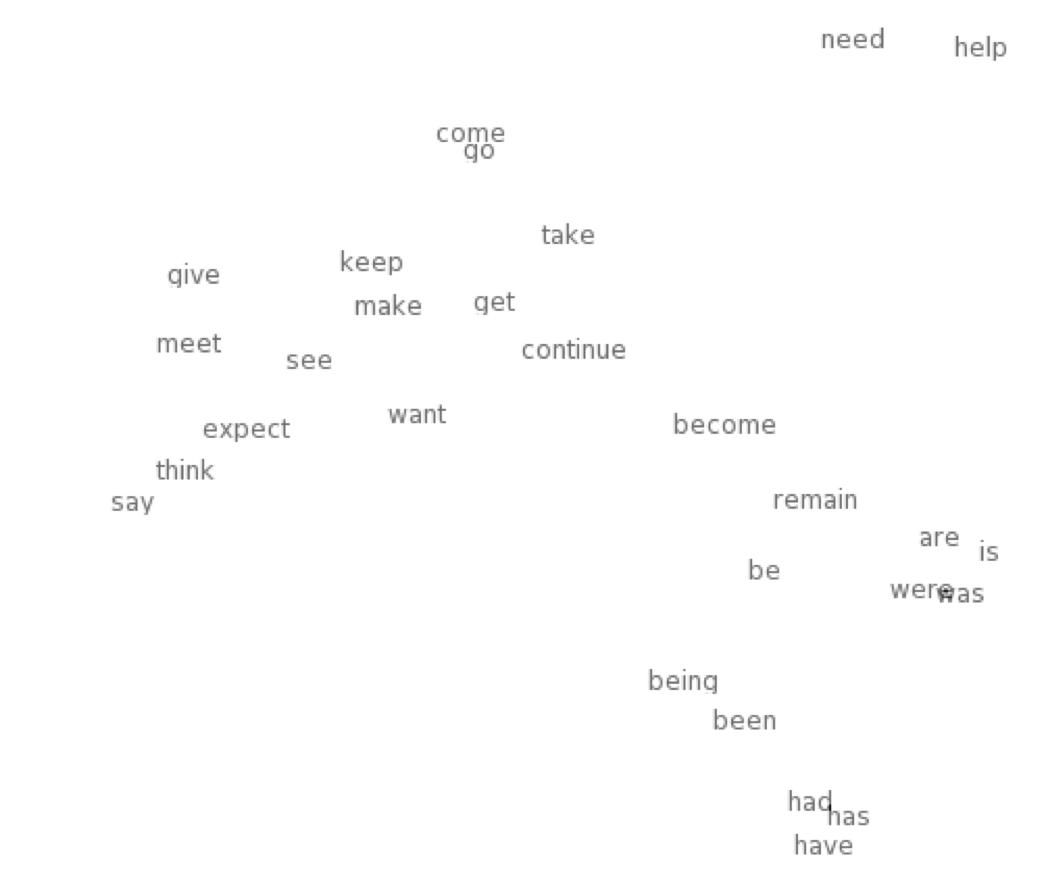
\includegraphics[width=0.49\linewidth]{word-embeddings.png}
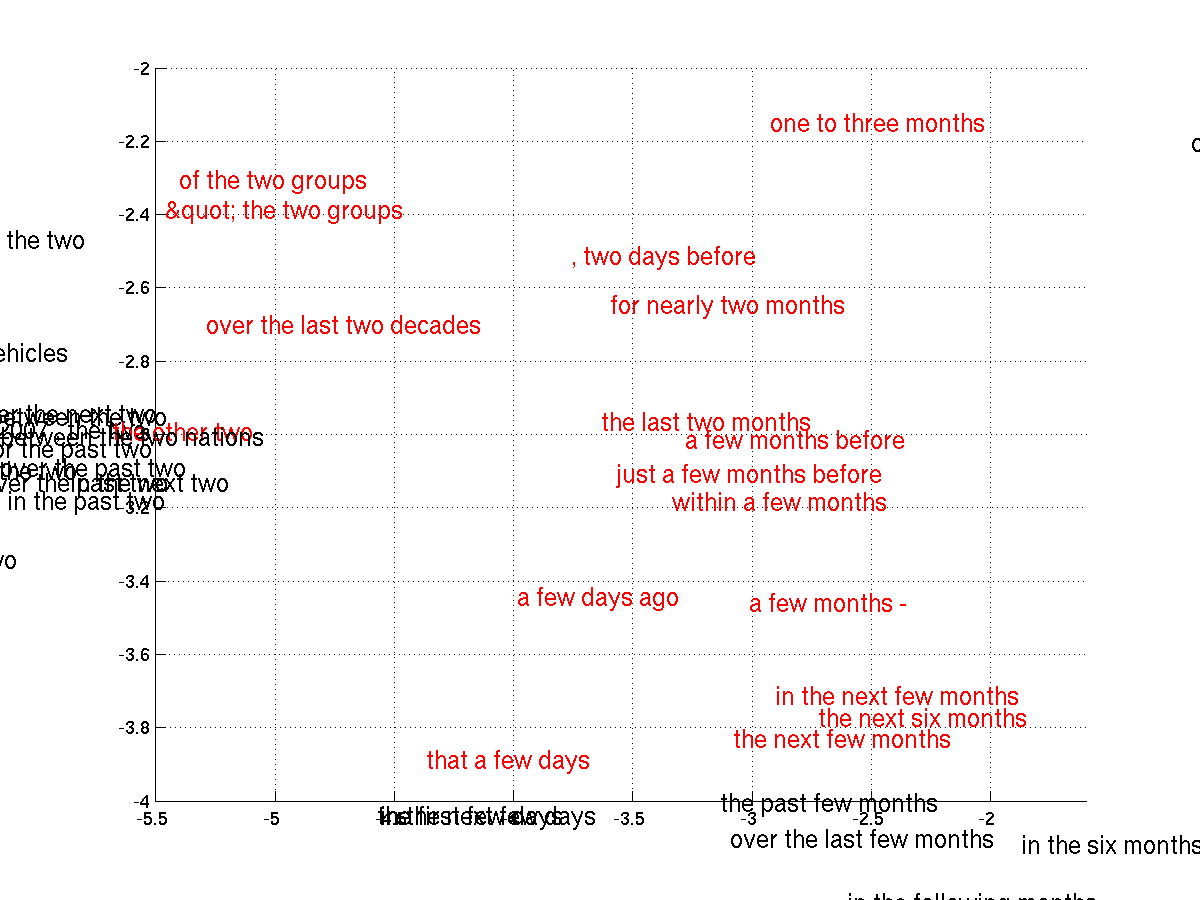
\includegraphics[width=0.49\linewidth]{phrase_zoom2.png}
}
\caption{Left: Illustration of word representations learned for modeling
language, non-linearly projected to 2-D for visualization using the
t-SNE algorithm~\citep{VanDerMaaten08}. Right: 2-D representation
of phrases learned by an English-to-French encoder-decoder recurrent
neural network~\citep{Cho-et-al-EMNLP2014}. One can observe that
semantically similar words or sequences of words are  mapped to
nearby representations.
}
\label{fig:word-embeddings}
\end{minipage}
}
\end{figure}

Instead of translating the meaning of a French sentence to an English sentence,
one can learn to ``translate'' the meaning of an image into an English sentence,
as illustrated in Figure~\ref{fig:caption-generation}. The ``encoder'' here is
a deep convolutional neural network which converts the pixels into an
activity vector in its last hidden layer. The ``decoder''
is a recurrent neural network similar to the ones used for machine translation
and neural language modeling. There has been a surge of interest in such
systems recently~\citep{Kiros-et-al-ICML2014,Mao+al-arxiv2014,Donahue-et-al-arxiv2014,
              Vinyals-et-al-arxiv2014,Fang-et-al-arxiv2014,
             Chen+Zitnick-arxiv2014,Karpathy+Li-arxiv2014,Venugopalan-et-al-arxiv2014}.

\begin{figure}[htp*]
\fbox{
\begin{minipage}{\textwidth}
\centerline{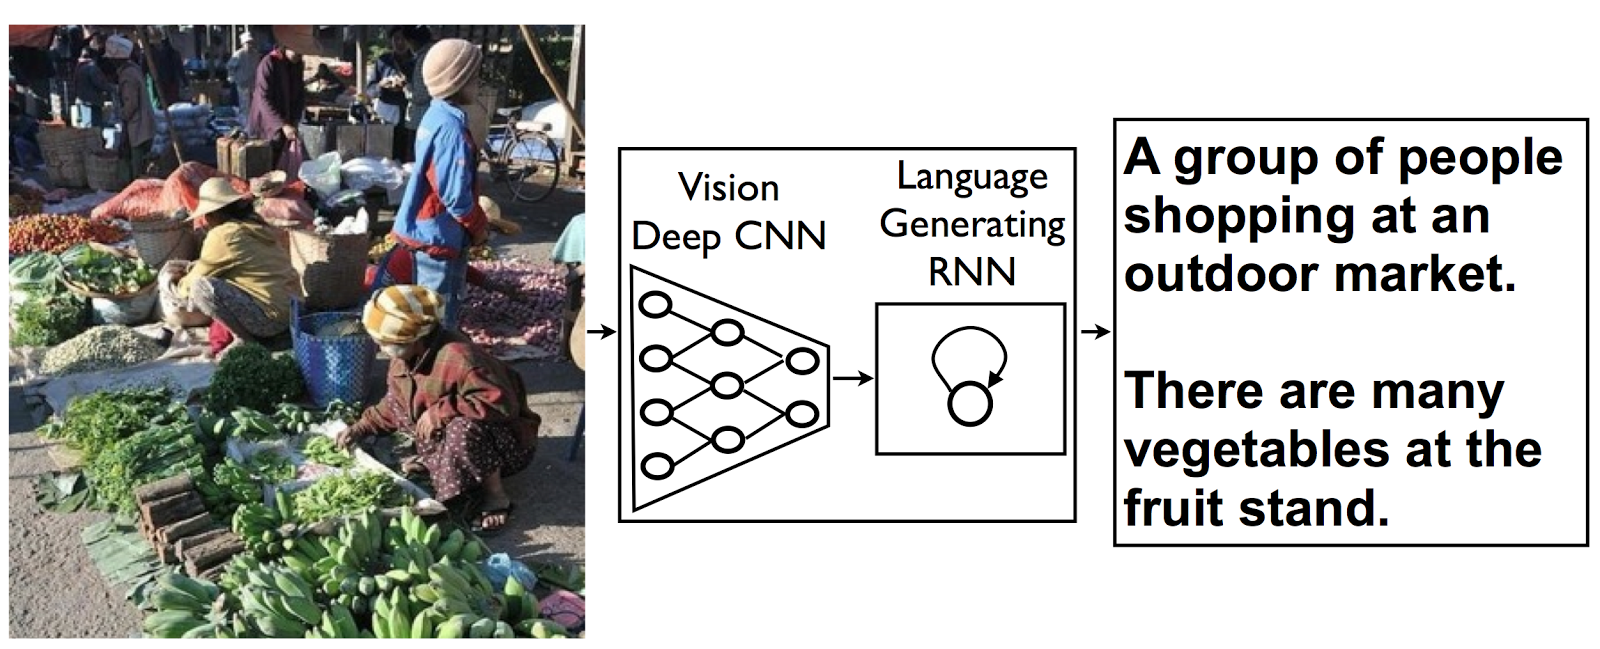
\includegraphics[width=\linewidth]{caption-generation-Vinyals-et-al.png}}
%\centerline{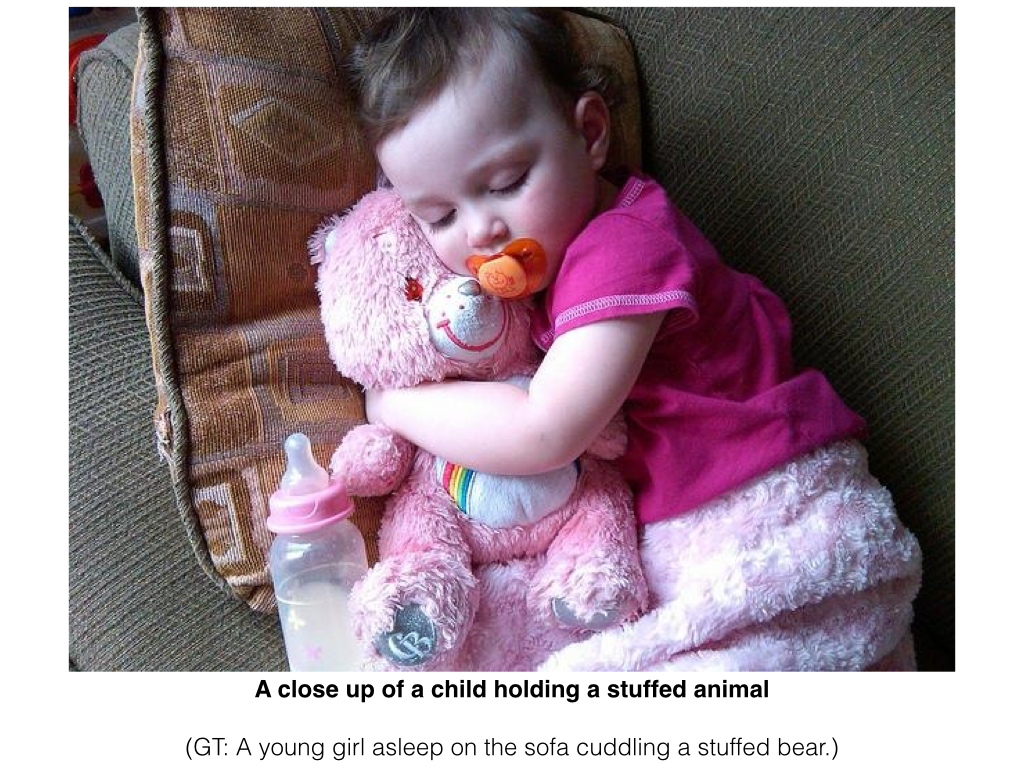
\includegraphics[width=0.49\linewidth]{Examples_im2txt_001.png}}
%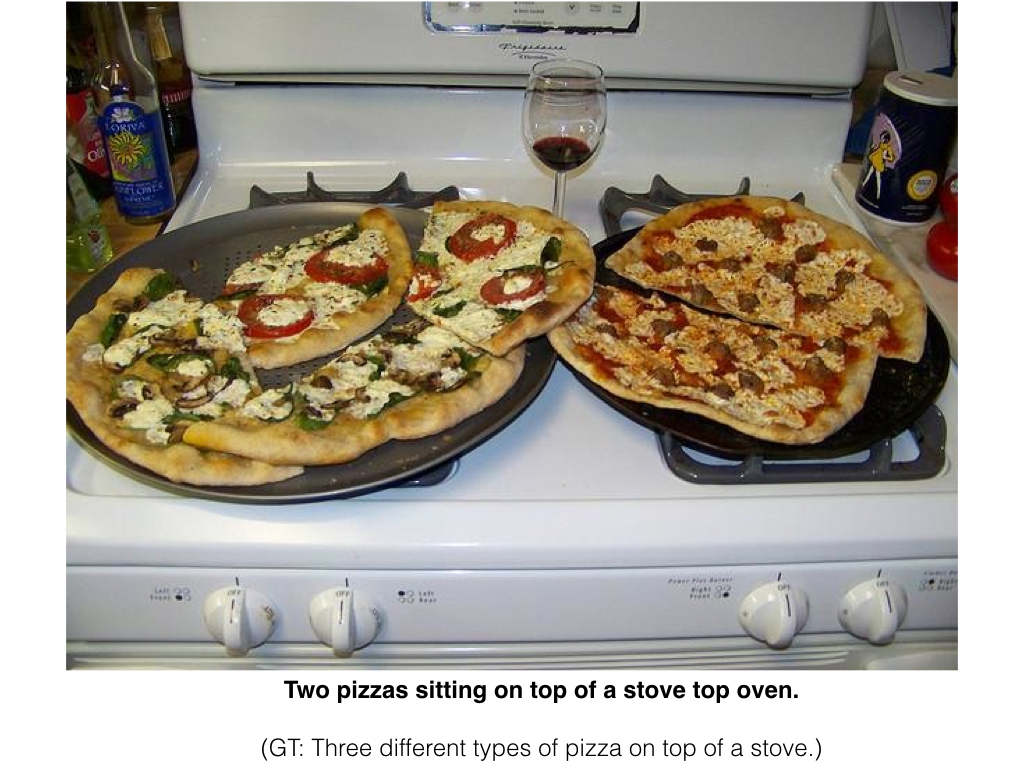
\includegraphics[width=0.49\linewidth]{Examples_im2txt_002.png}}
\centerline{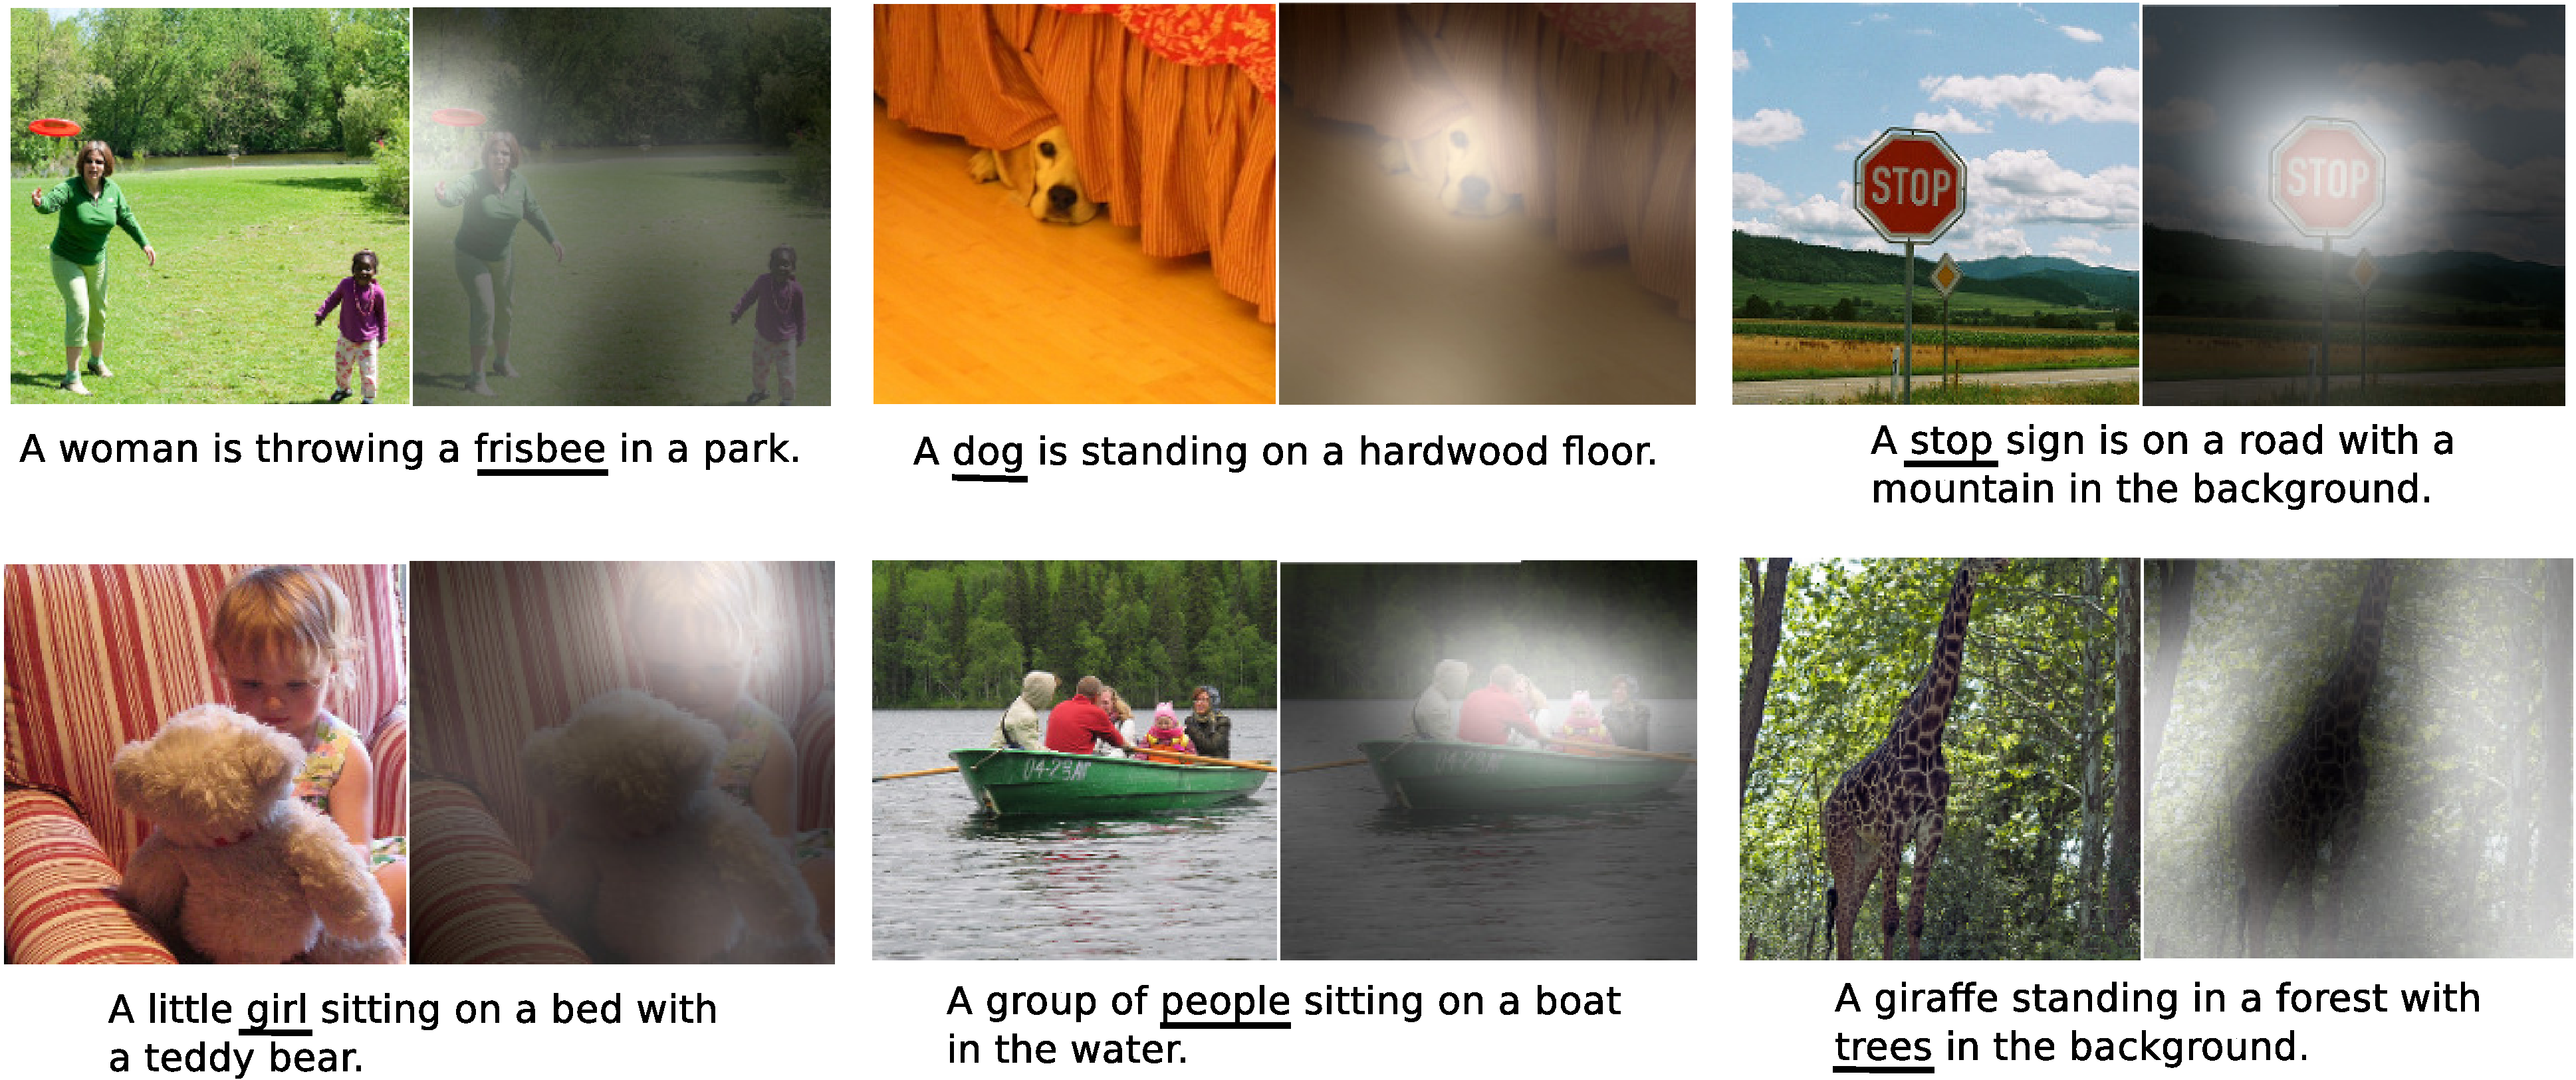
\includegraphics[width=\linewidth]{good_capgen_examples.pdf}}
%\centerline{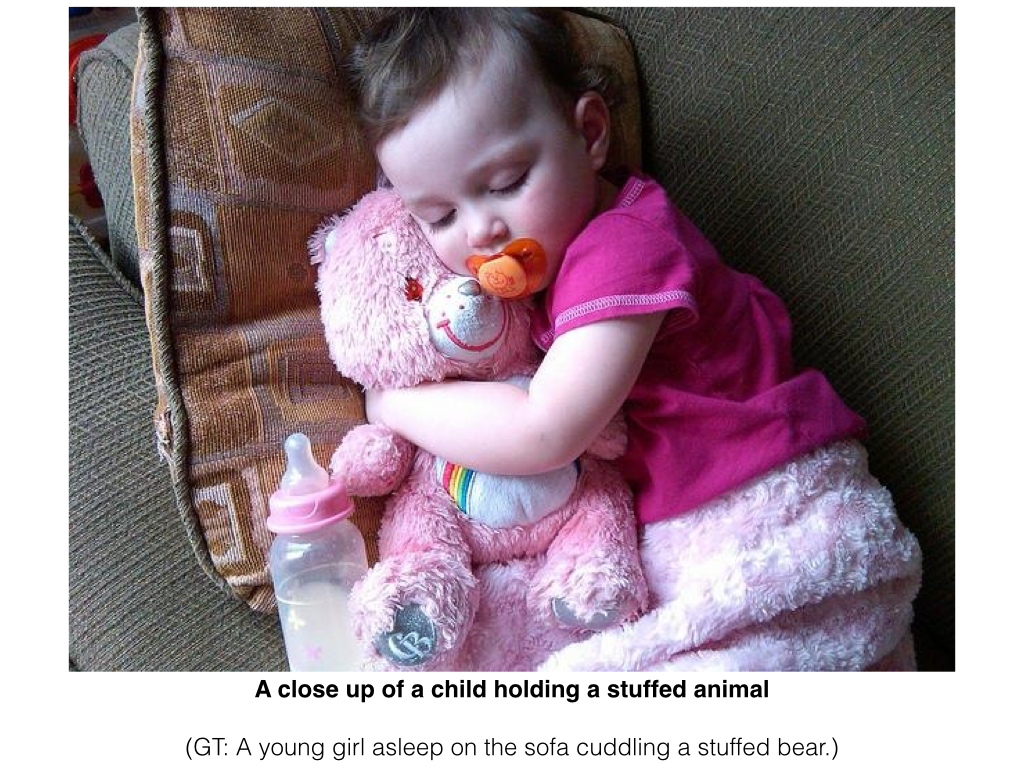
\includegraphics[width=0.49\linewidth]{Examples_im2txt_001.png}
\caption{Top: two examples of captions generated by a recurrent network taking
as extra input the representation extracted by a deep convolutional
net from a test image, with the recurrent network trained to ``translate''
high-level representations of images into captions. 
Reproduced with permission from~\citet{Vinyals-et-al-arxiv2014}.
Bottom: when the RNN is given the ability to focus its attention on a different
location in the input image (lighter = more attention) as it generates each word (underlined), we
found~\citep{Xu-et-al-arxiv2015} 
that it exploits this to achieve better ``translation'' of images into captions.
}
\label{fig:caption-generation}
\end{minipage}
}
\end{figure}



%%%%%%%%%%%%%%%%%%%% 

\section{Recurrent Neural Networks}
\label{sec:rnn}

When backpropagation was first introduced, its most exciting use was
for training recurrent neural networks. 
For tasks that involve sequential inputs, such as speech and language,
it is often better to use recurrent neural networks, illustrated in
Figure~\ref{fig:rnn}.  Recurrent neural networks process an input
sequence one element at a time, maintaining in their hidden units a
``state vector'' that implicitly contains information about the
history all the past elements of the sequence.  
When we consider the outputs of
the hidden units at different discrete time steps as if they were the
outputs of different neurons in a deep multi-layer network (right of
Figure~\ref{fig:rnn}), it becomes
clear how we can apply backpropagation to train recurrent
networks. The the gradient with respect to a recurrent weight,
$w_{ij}$ that allows neuron $i$ at time $t$ to influence the activity
of neuron $j$ at time $t+1$ can be computed by
backpropagation-through-time (BPTT) of the error derivative for $j$ at
time $t+1$. The full gradient with respect to $w_{ij}$ on a whole
input sequence is just the sum of its gradients at each time-step.

Recurrent neural networks are very powerful dynamical systems, but
training them with BPTT proved to be problematic, because the
backpropagated gradients either grow or shrink at each time step, so
over many time-steps they typically explode or
vanish~\citep{Hochreiter91-small,Bengio-et-al-TNN1994}.
%% THE TEXT BELOW IS TOO COMPLICATED AND ALSO TOO SIMPLE: THERE ARE
%% STABLE CONDITIONS IN WHICH THE GRADIENTS DO NOT VANISH (ORTHONORMAL
%% RECURRENT MATRICES). I THINK ITS BETTER NOT TO GET INTO THIS.
%% and the conditions which allow stable dynamics also correspond to
%% vanishing gradients~\citep{Bengio-et-al-TNN1994},

Thanks to advances in their architecture and ways of training them, recurrent networks 
have been found to be very good at predicting the next character in
text~\citep{Sutskever-et-al-ICML2011} or the next word in a
sequence~\citep{Mikolov-et-al-NIPS2013} but they can also be used for
more complex tasks.  After reading an English sentence one word at a
time, for example, an English ``encoder'' network can be trained so
that the final state vector of its hidden units is a good
representation of the thought expressed by the sentence.  This thought
vector can then be used as the initial hidden state of (or as extra
input to) a jointly trained French ``decoder'' network which outputs a
probability distribution for the first word of the French
translation. If a particular first word is chosen from this
distribution and provided as input to the decoder network it will then
output a probability distribution for the second word of the
translation and so on until a full stop is
chosen~\citep{Bahdanau-et-al-arxiv2014,Sutskever-et-al-NIPS2014}.
Overall, this process generates sequences of French words according to
a probability distribution that depends on the English sentence.

This rather naive way of performing machine translation has quickly become
competitive with the state-of-the-art and this raises serious doubts about
whether understanding a sentence requires anything like internal symbolic
expressions that are manipulated by binding their symbols to variables
in judiciously chosen rules of inference, as was previously thought by
many early AI researchers.  The encoder-decoder translation
networks do not work by using internal rules of inference in which
variables get bound to symbols. They just use big state vectors, big weight
matrices and scalar non-linearities to get the job done.  
Deriving conclusions using only the form of the premises (which is
what formal logic does) is a powerful
technique that people can eventually master, but the translation
results with recurrent neural networks suggest that it may not be a good model of
the way we normally reason or understand language. Recurrent neural
networks that represent thoughts as big vectors are more compatible with
the view that everyday reasoning involves many simultaneous analogies that
each contribute plausibility to a 
conclusion~\citep{Lakoff+Johnson-2008,Rogers+McClelland-book2004}.

\begin{figure}[htp*]
\fbox{
\begin{minipage}{\textwidth}
%\centerline{
%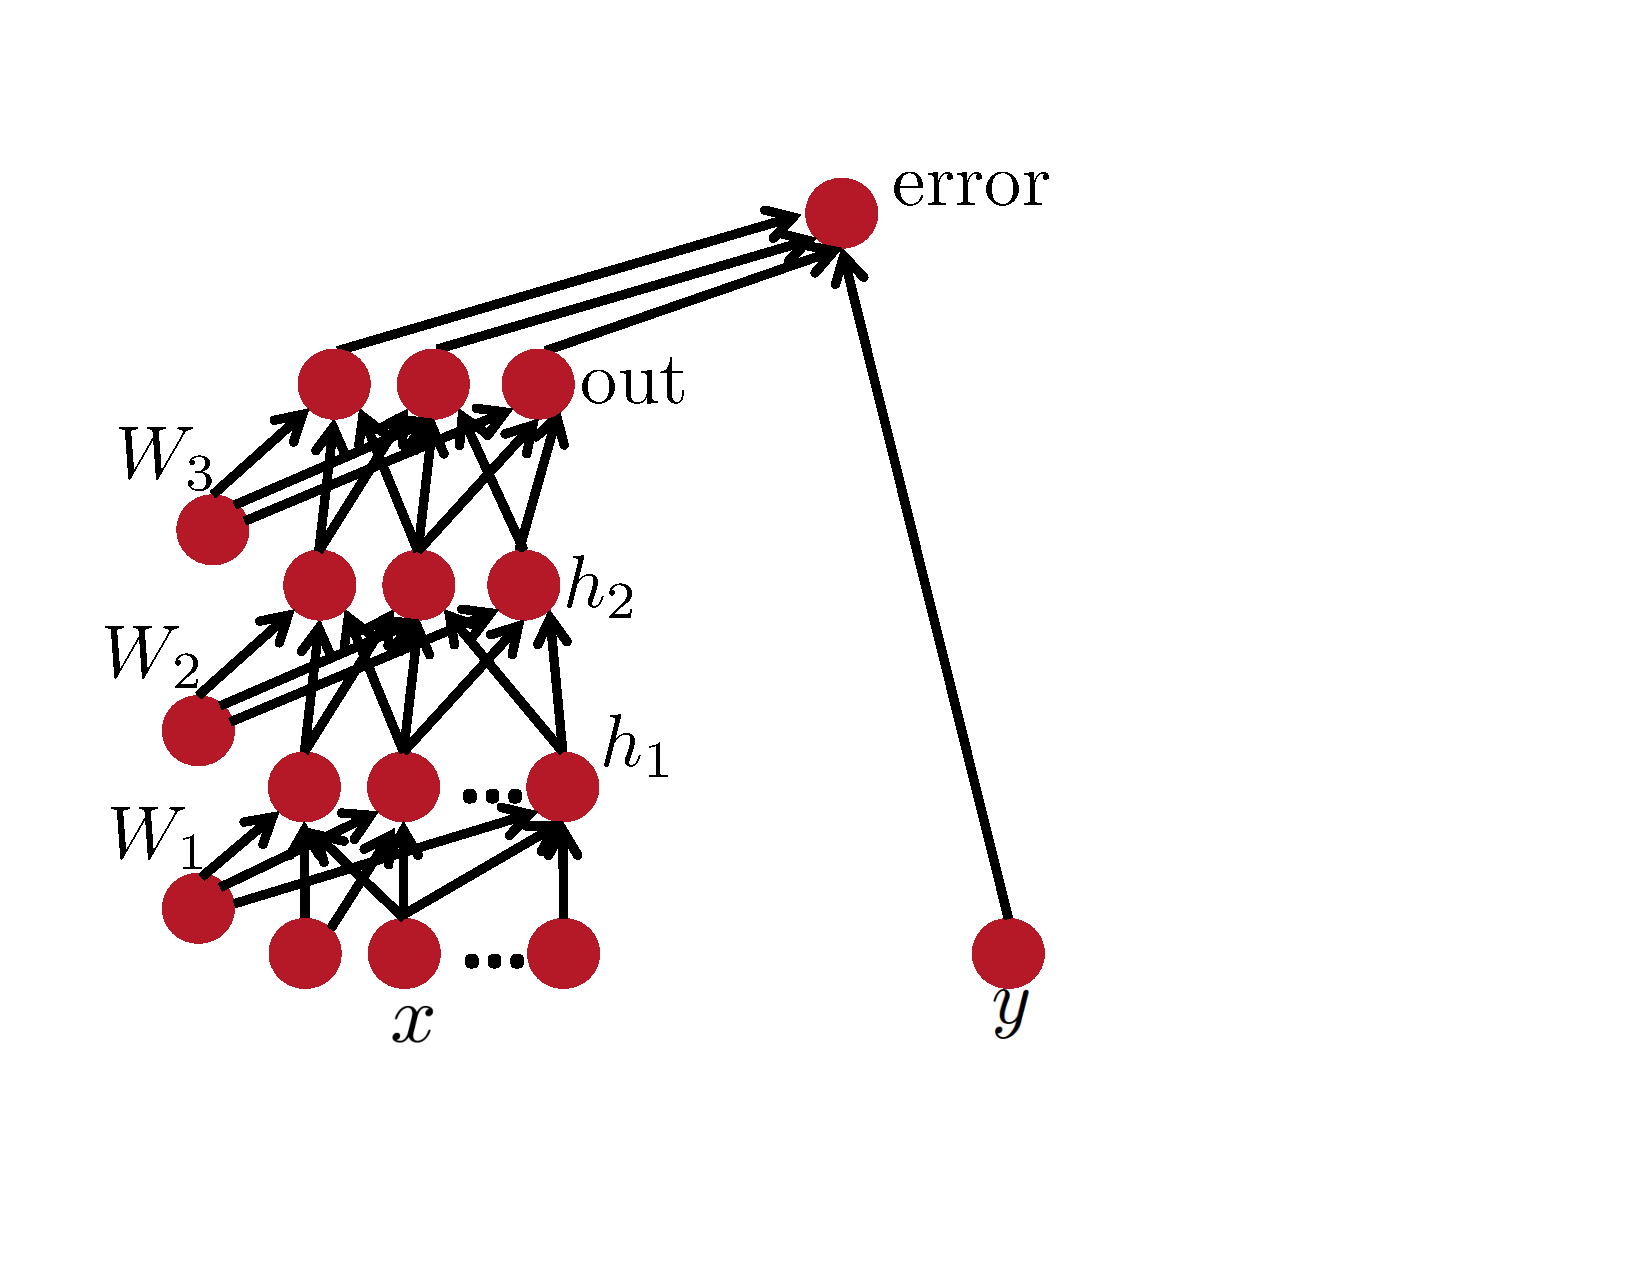
\includegraphics[width=0.49\linewidth]{bp-mlp1.pdf}
%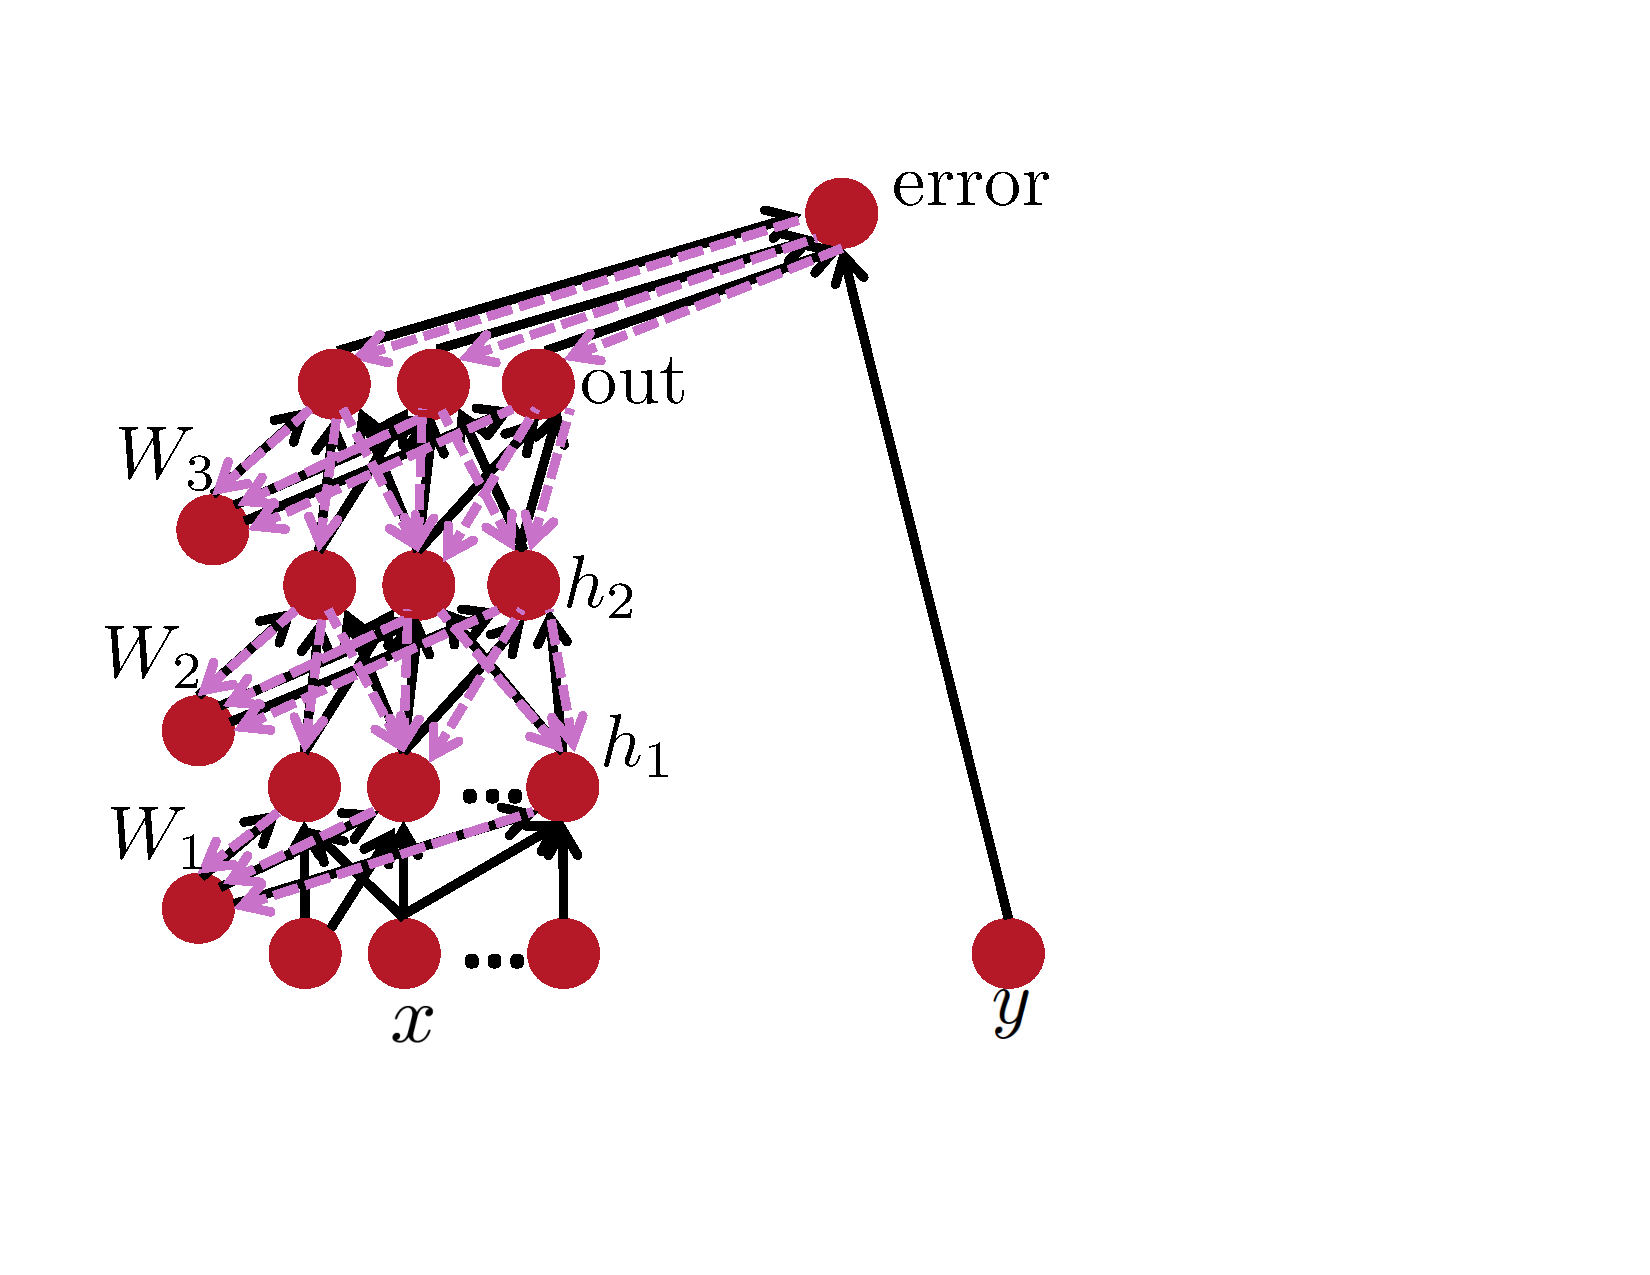
\includegraphics[width=0.49\linewidth]{bp-mlp5.pdf}
%}
\centerline{
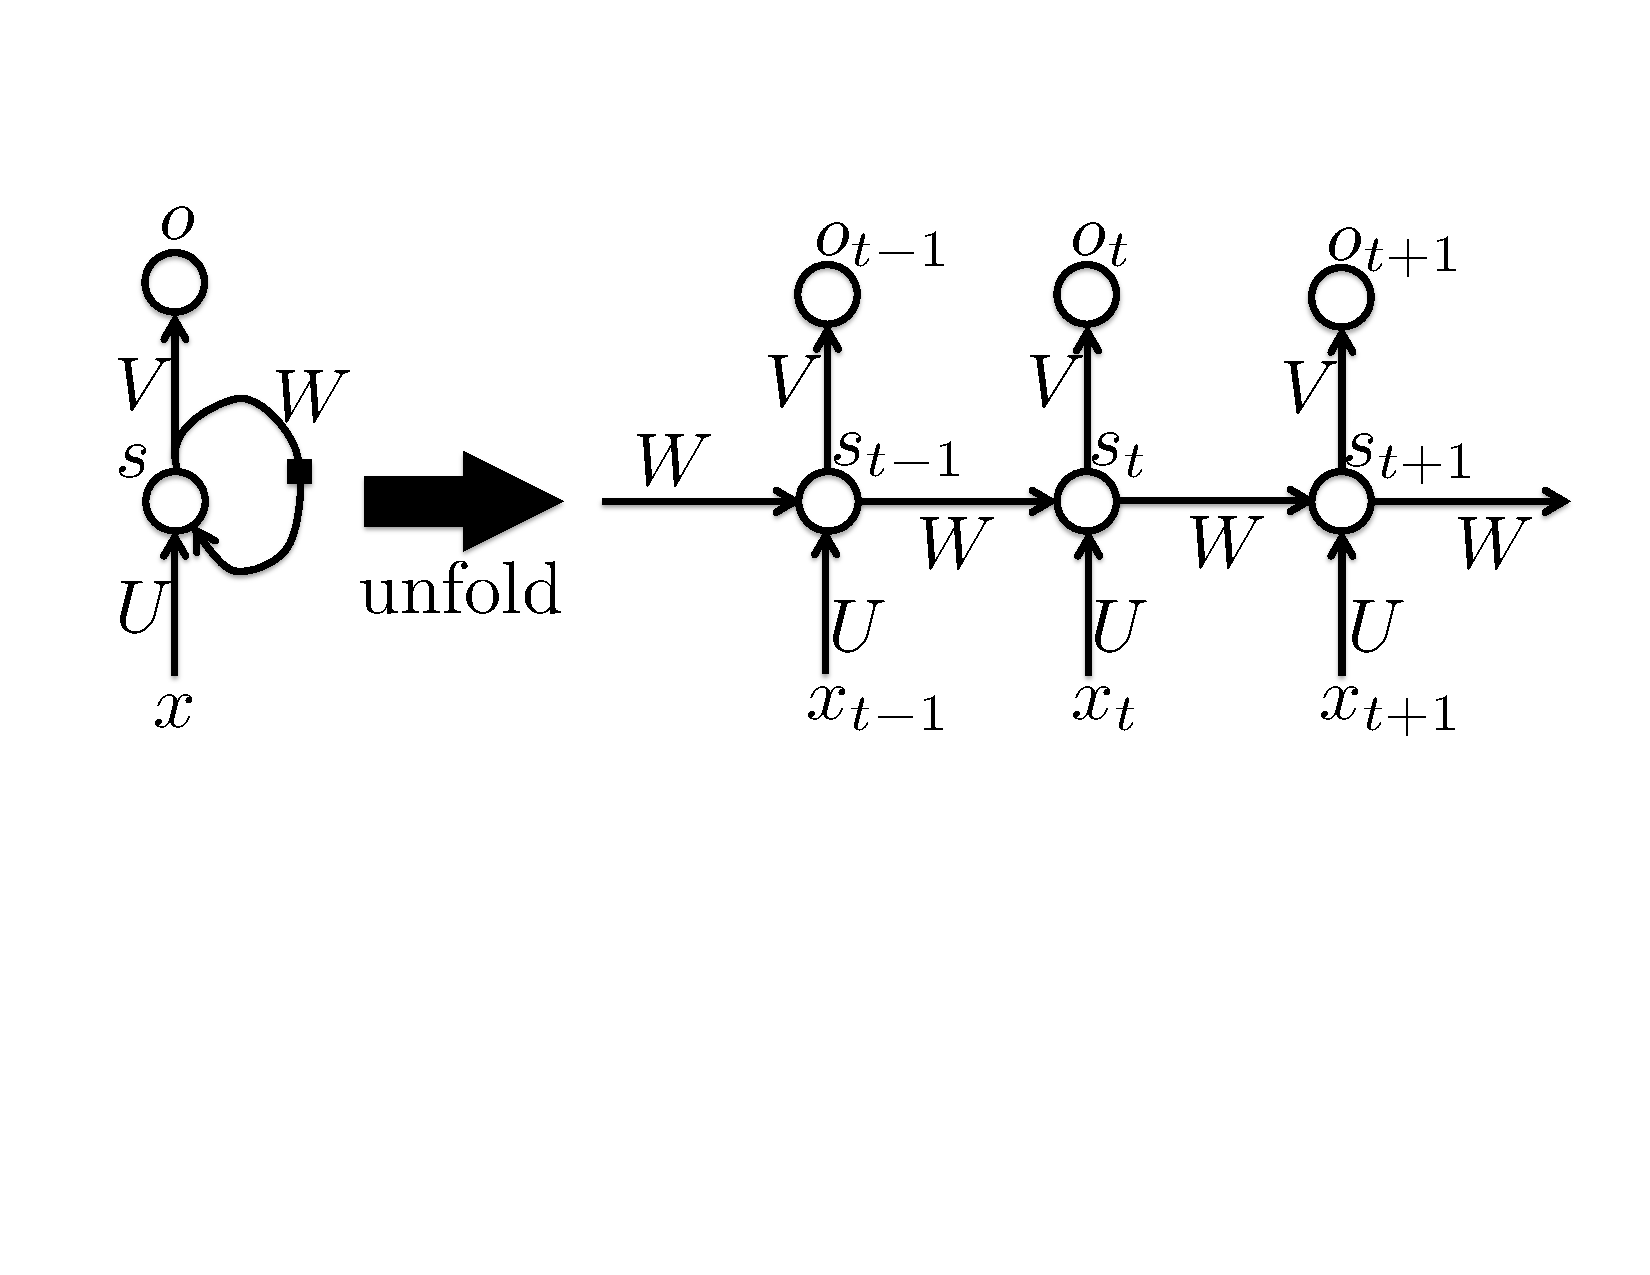
\includegraphics[width=0.89\linewidth]{fig-hidden-recurrence-rnn.pdf}
}
\caption{
%Top left: graph of feedforward computations in a multi-layer
%neural network with one input layer ($x$), two hidden layers ($h_1$ and $h_2$),
%one output layer (out), a target $y$, and an error that compares the output
%and the target. The synaptic weight matrices $W_1$, $W_2$ and $W_3$ are
%the parameters of the neural network.\newline
%Top right: back-propagation through the same multi-layer neural network
%(downward arrows compute the partial derivative of the error with respect
%to every node, i.e., the units value and the parameters).\newline
A recurrent neural network (left) and the unfolding in time of the
computation involved in its forward computation. The artificial neurons
(e.g. hidden units grouped under node $s$ with values $s_t$ at time $t$) 
get inputs from other neurons at previous time steps
(this is represented with the black square, standing for a delay of
one time step, on the left). In this way, a recurrent net can map an input sequence
with elements $x_t$ into an output sequence with elements $o_t$, with
each $o_t$ depending on all the previous $x_{t'}$ (for $t'\leq t$). The
same parameters (matrices $U$, $V$, $W$) are used at each time step.
Many other architectures are possible, including a variant in which
the sampled outputs (e.g. words) can be generated according to an output 
distribution (the probability of the next word, for every possible next word) 
and used as inputs for the next time step.
The back-propagation algorithm (Figure~\ref{fig:backprop-box})
can be directly applied to the computational graph of the unfolded network
on the right hand side, to compute the derivative of a total error
(e.g., the log-probability of generating the right sequence of
words) with respect to all the states $s_t$ and all the parameters.
}
\label{fig:rnn}
\end{minipage}
}
\end{figure}


\section{Recurrent Networks with Memory}
%% YLC: I moved this up because it connects with the RNN section above.

Recurrent networks, once unfolded in time, can be seen as very deep
feed-forward networks in which all the layers share the same weights.
While their main purpose is to learn long-term dependencies, they
don't actually seem to be able to store any information for very
long. The dynamics of the system is such that information about the
initial state vanishes quickly. 

To correct for that, one idea is to augment the network with an
explicit memory. The first proposal of this kind is the ``Long Short
Term Memory'' networks (LSTMs) that use special hidden units whose
natural behaviour is to remember inputs for a long
time~\citep{Hochreiter+Schmidhuber-1997}.  A linear ``memory cell''
interacts with other units via gated connections whose weights are
multiplied by the state of a logistic gating unit that takes a value
between $0$ and $1$. An input gating unit can learn when to isolate
the cell from the effect of the outside world, and an output gating
unit prevents the content of the memory cell to be broadcast to the
rest of the neural network. More importantly, the memory cell itself
acts like an accumulator or a gated leaky neuron: it has a connection
to itself at the next time-step that has a weight of 1 so it copies
its own real-valued state and accumulates the external signal, but
this self-connection is {\em gated} by a ``forget gate'' so the stored
value quickly leaks away unless the forget gate has an activation near
$1$.  The gates themselves have their activities determined by
weighted inputs that they receive from the input vectors and all of
the memory cells.

When LSTMs were first described \citep{Hochreiter+Schmidhuber-1997},
their complexity may have been off-putting and, despite their
impressive ability to learn very long-range temporal structure on toy
problems, they were largely ignored until they were shown to yield
excellent results in a cursive handwriting recognition
competition~\citep{Graves-et-al-2009}. They have subsequently proved
to be very effective for tasks that have sequential input.  When they
use several hidden layers, they are better than deep feedforward
networks for speech recognition~\citep{Graves-et-al-ICASSP2013} and
unlike feedforward nets they can implement an entire speech
recognition system that goes all the way from coefficents derived from
the soundwave to the sequence of characters in the transcription.
LSTMs or related forms of gated units are also what is currently used
for the encoder and decoder networks that perform so well at machine
translation~\citep{Bahdanau-et-al-arxiv2014,Sutskever-et-al-NIPS2014}.

Over the last year, several authors have made different proposals to
augment recurrent nets with a memory module. This includes simplified
version of the LSTM
circuit~\citep{Chung-et-al-NIPSDL2014-small,Yao-et-al-SLU-workshop2014}.
The results suggest that not all the elements of the LSTM architecture
are required.


Other proposals include the ``Neural Turing Machine'' in which the
network is augmented by a ``tape-like'' memory that the recurrent net
can chose to read from or write to~\citep{Graves-et-al-arxiv2014}, and
the ``Memory Network'' in which a regular network is augmented by a
kind of associative memory~\citep{weston-memorynet-2014}. Memory
networks have yielded excellent performance on standard
question-answering benchmarks. The memory is used to remember the
story about which the network is asked to answer questions.


%It is not yet clear which aspects of the complicated architecture of LSTMs
%are really necessary. Memory cells are a good way of allowing the
%backpropagated error derivatives to neither explode nor vanish, but they
%are not the only way.  For example, recurrent nets with rectified linear
%hidden units that use the non-linear function $y=max(0,x)$ are much simpler
%than LSTMs and if the recurrent weight matrix is initialized to be close to
%the identity matrix they work about as well as LSTMs both for toy problems
%involving very long-range temporal structure and for real tasks like
%predicting the next word in text\citep{LeHinton}.


\section{Learning to reason and to manipulate symbols}

Beyond simple memorization, Neural Turing Machines and Memory Networks
are being used for task that would normally require to manipulate
symbols and to reason.

Neural Turing Machines can be taught ``algorithms''. Among other
things, they can learn to ouput a sorted list of symbols when its
input consists of an unsorted sequence in which each symbol is
accompanied by a real value that indicates its priority in the list.
To achieve this it must learn a sorting program purely from examples
of the input and output sequences~\citep{Graves-et-al-arxiv2014}.

Memory Networks can be trained to keep track of the state of the world
when they are told a story, so that they can answer questions about
the state of the world at the end of the story. Following a sequence
of actions in a virtual world described in words, in a scenario
similar to a text adventure game, the network is shown an
automatically0generate question and taught to produce the
corresponding answer (also generated automatically).  In one test
example, the network is shown a 15-sentence version of the Lord of The
Rings and correctly answers questions like ``where is Frodo now?''.
~\citep{weston-memorynet-2014}

A different system that also uses BPTT can learn to map the sequence
of characters in a simple program written in Python to the sequence of
characters that the program would
print~\citep{Zaremba+Sutskever-arxiv2014}.  Rather surprisingly, BPTT
can learn about {\it for loops} and can also learn to perform addition
and multiplication of strings containing several decimal
digits. Achieving this kind of behaviour seemed ludicrously optimistic
when BPTT was first proposed.

In a somewhat related work, a network is trained to evaluate whether a
particular mathematical transformation of a formula is lilely to lead
to a correct mathematical identity~\cite{zaremba-nips-2014}. The
system was able to produce efficient identities for matrix expressions
whose formula fill several pages.

The renewal of interest in deep learning and recurrent neural nets is
spurring a whole new generation of creative ideas.
  
\section{Deep reinforcement learning}

Learning which action will maximize the total future reward given a state
of the world is difficult when the rewards are delayed and the world has a
very large number of possible states. One impressive recent development is
a single system that can learn to play many different video
games~\citep{Deepmind-atari-arxiv2013}. The system uses a deep convolutional network to
map from the pixels on the screen at several time steps to the
expected future reward of each possible action and its only inputs are the
pixels and the current score in the game. The learning works by minimizing
the difference between the system's current estimate of future reward and a
noisy but less biased estimate that is obtained by using the same deep
network to estimate the future reward of the next state, where the next
state is chosen stochastically based on the predicted future rewards of all
the currently legal actions.


\section{Overcoming the limitations of backpropagation}

In the late 1990s, neural nets and backpropagation were largely
forsaken by the machine learning community. At the time, people
believed that learning many layers of non-linear feature detectors
with no prior knowledge was much too difficult for a simple gradient
descent procedures and that the networks were getting trapped in poor
local minima, weight configurations for which no small change would
reduce the average error, despite considerable empirical evidence to
the contrary in the case of ConvNets~\citep{lecun-98}. We now know
that the main reasons for the limited success of backpropagation in
deep networks were quite different: labeled datasets that were often
too small, computers that were too slow, non-linearities that were
inappropriate, weights that were not properly
initialised~\citep{lecun-98b,GlorotAISTATS2010-small}, and a lack of
faith in the potential success.

The obvious perceived weakness of stochastic gradient descent is that
it can get trapped in poor local minima, but it turns out that local
minima are rarely a problem with large networks. Regardless of the
initial conditions, the system always reaches solutions of similar
quality.  Recent results strongly suggest the landscape is packed with
a combinatorially large number of {\em saddle points} where the
gradient is zero, and the surface curves up in some dimensions and
curves down in
others~\citep{Dauphin-et-al-NIPS2014-small,Choromanska-et-al-AISTATS2015}.
The analysis seems to show that the local minima are present in very
large numbers, but almost all of them have very similar error levels.
Hence it doesn't seem to matter which one the algorithm
finds. Avoiding being trapped near saddle points seems more important.

It also took an inordinate amount of time for the community to adopt
stochastic gradient methods for large-scale machine learning. key
theoretical and practical work showed that, while SGD has terrible
asymptotic convergence properties, it is extremely efficient for the
kind of approximate optimization required in ML
applications~\citep{bottou-bousquet-2008-small}. But when trainnig a
large ConvNet can take days or weeks on the fastest GPUs, one is eager
to discover more efficient optimization methods that use the curvature
information the past update directions~\citep{lecun-98b,Montavon2012}.

The parallelization of large neural nets over a single GPU has
required to use ``mini-batches'' of samples over which the gradients
are averaged. The purpose of this is to saturate the GPU. But one big
unsolved question is how to scale up the training of very large neural
nets over multiple GPU card across multiple machines. As of today, this
question is unresolved.

Interest in deep feedforward networks was revived around
2006~\citep{IJCAI,Hinton06-small,Bengio-nips-2006-small,ranzato-07-small}
by the introduction of unsupervised learning procedures that could
create layers of feature detectors without requiring labeled data. The
objective in learning each layer of feature detectors was to be able
to reconstruct or model the activities of feature detectors (or raw
inputs) in the layer below.  By ``pre-training'' several layers of
progressively more complex feature detectors using this reconstruction
objective, the weights of a deep network could be initialized to
sensible values.  A final layer of output units could then be added to
the top of the network and the whole deep system could be fine-tuned
using standard backpropagation
\citep{Hinton-Science2006,Bengio-nips-2006-small,ranzato-07-small}.
This worked remarkably well for recognizing handwritten digits or for
detecting pedestrians, especially when the amount of labeled data was
very limited~\citep{Erhan+al-2010-small,sermanet-cvpr-13}.

The first major application of this pre-training approach was in
speech recognition and it was made possible by the advent of fast
Graphics Processing Units (GPUs) that were convenient to
program~\citep{RainaICML09-small} and allowed researchers to train
networks 10 or 20 times faster.  In 2009, the approach was used to map
short temporal windows of coefficients extracted from a soundwave to a
set of probabilities for the various fragments of speech that might be
represented by the frame in the center of the window.  It achieved
record-breaking results on a standard speech recognition benchmark
that used a small vocabulary~\citep{TIMITpaper} and was quickly
developed to give record-breaking results on a large vocabulary
task~\citep{Dahl2012}.  By 2012, versions of the deep net from 2009
were being developed by many of the major speech
groups~\citep{Hinton-et-al-2012} and were already being deployed in
Android phones.  For smaller datasets, unsupervised pre-training helps
to prevent overfitting~\citep{Erhan+al-2010-small}, leading to
significantly better generalization when the number of labeled
examples is small, or in a transfer setting where we have lots of
examples for some ``source'' tasks but very few for some ``target''
task. In this context, unsupervised representation learning helped to
win several transfer learning
competitions~\citep{UTLC+LISA-2011-small,Goodfellow-icml2012}.  Once
deep learning had been rehabilitated, it turned out that large labeled
datasets did not need the pre-training stage. Even better results,
especially for very deep networks, could be obtained by using
rectifying non-linearities rather than sigmoid or tanh non-linearities
~\citep{Nair-2010-small,Glorot+al-AI-2011-small,Krizhevsky-2012-small,Dahl-et-al-ICASSP2013}.


\section{The future of deep learning}

Human vision is an active process in which intelligent fixations are
used to ensure that only a tiny fraction of the optic array is ever
processed at high resolution. We expect much of the future progress in
vision, especially for video understanding or robotics, to come from
systems that are trained end-to-end and combine deep convolutional
networks with recurrent nets that use reinforcement learning to decide
where to look.  Such systems already outperform passive vision
systems~\citep{ba+mnih}.  Similarly, when understanding sentences or
whole documents we expect future systems to learn strategies for
selectively attending to one part at a
time~\citep{Bahdanau-et-al-arxiv2014}. We also expect that in the next
few years deep recurrent neural networks will become far better at
understanding the meaning of documents, including the way in which the
thoughts expressed by the sentences are related to one another.

This review has focused on supervised learning because of its recent
achievements and we have ignored much interesting work on unsupervised
learning procedures for deep neural
networks~\citep{Salakhutdinov2009-small,Hinton95,QuocLe-ICML2012,VincentPLarochelleH2008-small,koray-nips-10,gregor-icml-10,ranzato-pami,Bengio-et-al-ICML-2014,Kingma-et-al-NIPS2014}.
However, most data have not been hand-labeled by humans, and just like
children are not told what they should have done at each instant, we
need learning machines that can learn from mostly unlabeled examples.
In the long run, we believe unsupervised learning will be essential
for allowing deep networks to generalize well by creating internal
representations that untangle the many different factors that interact
to produce images, speech and
documents~\citep{Bengio-Courville-Vincent-TPAMI2013}.

We expect to see more innovative ideas that marry deep learning with
reasoning. Reasoning can be formulated in a number of different ways:
energy minimization, contraint satisfaction, chains of operations
applied to vectors representing objects or symbols. One is hoping for
an architecture that unifies representation learning with
reasoning~\citep{bottou-mlj-2014}.

Finally, we believe that the recent successes of deep learning using
stochastic gradient descent are only the beginning.  As pointed out
in~\citet{Bengio+Lecun-chapter2007-small}, end-to-end learning
systems that have many parameters and few built-in assumptions can make use
of more data and more compute power far more easily than systems that
require hand-engineering of domain-specific knowledge.

 
%\section{Key references}
%{\it Quite a few of these are very recent and have not yet been published
%  through a peer-review so we are giving their arxiv references}.





%\subsection{Back-propagation and Stochastic Gradient Descent}

%Rumelhart, D. E., Hinton, G. E., \& Williams, R. J. (1986)\\ Learning
%representations by back-propagating errors.\\ {\it Nature}, {\bf 323},
%533-536.
% --> \citep{Rumelhart86b}

%LeCun, Y., Boser, B., Denker, J. S., Henderson, D., Howard, R.E., Hubbard,
%W., \& Jackel, L.D.\\ Backpropagation Applied to Handwritten Zip Code
%Recognition\\ Neural Computation, 1(4):541-551, Winter 1989
%--> \citep{LeCun89-small}

%\subsection{Distributed representations}

%Hinton, G. E., McClelland, J. L., \& Rumelhart, D. E. (1986)\\ Distributed
%representations.\\ In Rumelhart, D. E. and McClelland, J. L., editors, {\it
%  Parallel Distributed Processing: Explorations in the Microstructure of
%  Cognition. Volume 1: Foundations}, MIT Press, Cambridge, MA. pp 77-109.
% --> \citep{Hinton-et-al-PDP1986}

%Bengio, Y., Ducharme, R., \& Vincent, P. (2001)\\ A neural probabilistic
%language model.\\ In {\it NIPS 2000}, pages 932--938.
% --> \citep{BenDucVin01-short}

%% Collobert, R., Weston, J., Bottou, L., Karlen, M., Kavukcuoglu, K., Kuksa, P. (2011)\\
%% Natural language processing (almost) from scratch.\\
%% {\it The Journal of Machine Learning Research} 12, pages 2493-2537
% --> \citep{collobert:2011b}

%Mikolov, T., Sutskever, I., Chen, K., Corrado, G.S., \& Dean
%J.\\ Distributed representations of words and phrases and their
%compositionality.\\ In {\it NIPS 2013}, pages 3111-3119.
% --> \citep{Mikolov-et-al-NIPS2013}

%Montufar, G.~F., Pascanu, R., Cho, K., and Bengio, Y. (2014).  On the
%number of linear regions of deep neural networks.\\ In {\it NIPS'2014}.
% --> \citep{Montufar-et-al-NIPS2014}.

%\subsection{The apparent limitations of backpropagation in deep networks}

%Bengio, Y., Simard, P., \& Frasconi, P. (1994)\\ Learning long-term
%dependencies with gradient descent is difficult.\\ {\it IEEE Transactions
%  on Neural Networks}, 5(2), 157-166.
% --> \citep{Bengio-et-al-TRNN1994}

%% Dauphin, Y., Pascanu, R., Gulcehre, C., Cho, K., Ganguli, S., and Bengio,
%% Y.\\ 
%% Identifying and attacking the saddle point problem in high-dimensional
%% non-convex optimization.\\ In {\it NIPS'2014}.

%\subsection{Deep unsupervised learning}
%Hinton, G., Osindero, S., \& Teh, Y. W. (2006)\\ A fast learning algorithm
%for deep belief nets.\\ {\it Neural Computation}, 18(7), 1527-1554.
% --> \citep{Hinton06-small}

%Erhan, D., Bengio, Y., Courville, A., Manzagol, P. A., Vincent, P., \&
%Bengio, S. (2010)\\ Why does unsupervised pre-training help deep
%learning?\\ {\it The Journal of Machine Learning Research}, {\bf 11},
%625-660.
% --> \citep{Erhan+al-2010-small}

%% Mesnil, G., Dauphin, Y., Glorot, X., Rifai, S., Bengio, Y., Goodfellow, I.,
%% Lavoie, E., Muller, X., Desjardins, G., Warde-Farley, D., Vincent, P.,
%% Courville, A., and Bergstra, J. (2011).\\ Unsupervised and transfer learning
%% challenge: a deep learning approach.\\ In {\em JMLR W\&CP: Proc. Unsupervised
%%  and Transfer Learning\/}, volume~7.

%\subsection{Deep speech recognition}

%% Mohamed, A. R., Dahl, G. E., \& Hinton, G. (2012)\\ Acoustic modeling using deep
%% belief networks.\\ {\it IEEE Transactions on Audio, Speech, and Language
%%  Processing}, 20(1), 14-22.

%Hinton, G., Deng, L., Yu, D., Dahl, G. E., Mohamed, A. R., Jaitly, N. \&
%Kingsbury, B. (2012)\\ Deep neural networks for acoustic modeling in speech
%recognition: The shared views of four research groups.\\ {\it Signal
%  Processing Magazine}, IEEE, 29(6), 82-97.
% --> \citep{Hinton-et-al-2012}


%\subsection{Deep convolutional networks for image understanding}
%LeCun, Y., Bottou, L., Bengio, Y., \& Haffner, P. (1998)\\ Gradient-based
%learning applied to document recognition.\\ {\it Proceedings of the IEEE},
%86(11), 2278-2324.
% --> \citep{LeCun+98}

%% Jain, V., Seung, H.S., \& Turaga S.C. (2010)\\
%% Machines that learn to segment images: a crucial technology for connectomics\\
%% {\it Current opinion in neurobiology} 20 (5), 653-666.

%Krizhevsky, A., Sutskever, I., \& Hinton, G. E. (2012)\\ Imagenet
%classification with deep convolutional neural networks.\\ In Advances in
%Neural Information Processing Systems (1097-1105).
% --> \citep{Krizhevsky-2012-small}

%% Farabet, C., Couprie, C., Najman, L. \& LeCun, Y. (2013)\\
%% Learning Hierarchical Features for Scene Labeling,\\
%% IEEE Transactions on Pattern Analysis and Machine Intelligence, August 2013.

%% Sermanet, P., Eigen, D., Zhang, X., Mathieu, M., Fergus, R., \& LeCun,
%% Y. (2013)\\ Overfeat: Integrated recognition, localization and detection using
%% convolutional networks.\\ {\it Proceedings of ICLR 2014}, arXiv:1312.6229.

%Tompson, J., Goroshin, R., Jain, A., LeCun, Y., \& Bregler, C. (2014)
%Efficient Object Localization Using Convolutional
%Networks. arXiv:1411.4280.
% --> \citep{Tompson-et-al-arxiv2014}

%\subsection{Deep recurrent neural networks for text understanding and machine translation}

%Graves, A., Liwicki, M., Fernández, S., Bertolami, R., Bunke, H., \&
%Schmidhuber, J. (2009)\\ A novel connectionist system for unconstrained
%handwriting recognition.\\ {\it IEEE Transactions on Pattern Analysis and
%  Machine Intelligence}, 31(5), 855-868.
% --> \citep{Graves-et-al-2009}

%% Devlin, J., Zbib, R., Huang, Z., Lamar, T., Schwartz, R., \& Makhoul,
% J. (2014)\\ Fast and robust neural network joint models for statistical machine
%% translation.\\ In {\it 52nd Annual Meeting of the Association for Computational
%%   Linguistics}, Baltimore, MD, USA.

%Sutskever, I., Vinyals, O., \& Le, Q. V. (2014)\\ Sequence to sequence
%learning with neural networks.\\ {\it arXiv preprint}, arXiv:1409.3215.


% --> \citep{Sutskever-et-al-NIPS2014}

%Bahdanau, D., Cho, K., \& Bengio, Y. (2014)\\ Neural machine translation by
%jointly learning to align and translate.  {\it arXiv preprint},
%arXiv:1409.0473.
% --> \citep{Bahdanau-et-al-arxiv2014}

%Vinyals, O., Toshev, A., Bengio, S., \& Erhan, D. (2014)\\ Show and Tell: A
%Neural Image Caption Generator.\\ {\it arXiv preprint}, arXiv:1411.4555.
% --> \citep{Vinyals-et-al-arxiv2014}


%% Weston, J., Chopra, S., Bordes, A. (2014)\\
%% Memory Networks. arXiv:1410.3916.

%\subsection{Deep reinforcement learning}
%Mnih, V., Kavukcuoglu, K., Silver, D., Graves, A., Antonoglou, I.,
%Wierstra, D., \& Riedmiller, M. (2013)\\ Playing Atari with deep
%reinforcement learning.\\ {\it arXiv preprint} arXiv:1312.5602.
% --> \citep{Deepmind-atari-arxiv2014}

%\newpage

\iffalse
\section{Boxes (TODO)}

A box for the forward propagation and backpropagation equations.

\section{Figures}

1. Diagram showing:\\ a) A feedforward neural net.\\ b) A recurrent neural
net expanded in time.\\ c) A convolutional neural net.

DONE 2. Maps showing:\\ a) that word vectors learned by backpropagation are very
good at capturing the meanings of the words.\\ b) that the thought vectors
extracted by a translation model are very good at capturing the thoughts
expressed by sentences.

3. A diagram showing how unsupervised learning can be used to pre-train a
deep feeedforward neural net.

4. Some images with:\\ a) The opinions of a deep convolutional net about
the classes of the prominent objects.\\ 
DONE b) Several alternative captions
generated by using the output of the convolutional net to determine the
initial hidden state of a decoder recurrent net.
 
5. Some images showing the localizations of parts of a person found by a
deep convolutional neural net.\\

\fi

\bibliography{strings,ml,aigaion,convnetyann,lecun}
\bibliographystyle{natbib}

\end{document}


